% DOCX paragraph 455
\chapter[Estrellas de neutrones]{Estrellas de neutrones: las maravillas de la física}\label{ch:05}

% DOCX paragraph 458
En los capítulos 3 y 4 exploramos los conceptos de espaciotiempo y curvatura y vimos cómo esta última da lugar a la gravedad. También nos detuvimos a reflexionar sobre cómo el espaciotiempo es a la vez elástico y muy rígido, y verificamos que la curvatura en la Tierra es extraordinariamente pequeña (lo cual explica por qué tendemos a pensar en términos de espaciotiempo plano). Por último, mediante un experimento mental, concluimos que es posible obtener curvaturas considerables concentrando grandes cantidades de masa (o energía) en volúmenes diminutos; por ejemplo, «encogiendo» el radio del Sol hasta diez kilómetros. Ahora ha llegado el momento de descubrir juntos en qué circunstancias es la naturaleza capaz de producir aquello que planteamos como hipótesis en nuestro experimento mental.

% DOCX paragraph 459
Pero para llegar hasta allí es necesario que demos un paso atrás en el tiempo y volvamos al conocimiento que se tenía del universo a finales de la década de 1950 y principios de la de 1960. En aquella época, los científicos habían alcanzado una comprensión precisa de los procesos termonucleares que tienen lugar dentro de las estrellas y les permiten producir energía mediante la fusión de elementos ligeros, como el hidrógeno y el helio, convirtiéndolos en elementos cada vez más pesados, tales como el carbono, el nitrógeno y el oxígeno, e incluso otros más pesados aún, como el níquel y el hierro. El conocimiento general sobre este tema, fruto de una fascinante colaboración entre la física nuclear, la física gravitatoria y la astronomía, había infundido gran confianza a los científicos, quienes se habían convencido de que comprendían el funcionamiento de los objetos estelares.

% DOCX paragraph 460
Se trataba de un marco teórico extremadamente complejo que precisaba una gran cantidad de conocimientos para analizar detalladamente los procesos nucleares que tienen lugar en las profundidades más inaccesibles de las estrellas (y también para seguir los numerosos caminos evolutivos que pueden tomar según su edad y composición). No obstante, la impresión básica era que la astrofísica nuclear y la astronomía habían llegado a ser capaces de reconstruir y explicar los numerosos escenarios que contemplaba la astrofísica estelar. Por tanto, el ambiente que reinaba en la comunidad científica reflejaba la convicción de que, con excepción de unos pocos aspectos menos claros, el panorama general de la astrofísica estelar estaba prácticamente completo y esencialmente controlado. Todas las observaciones realizadas hasta entonces eran, de hecho, perfectamente compatibles con el progreso en el estudio de las partículas elementales y con lo que se sabía en esos años de la física moderna. Finalmente, en lo que respecta a la gravedad, la teoría de Newton, consagrada por el tiempo, proporcionaba todos los elementos necesarios para describir los fenómenos físicos de las estrellas, tanto para objetos como el Sol como para otros con masas incluso cien veces mayores. Por supuesto que también se podía invocar la teoría de la gravedad de Einstein, pero la mayoría la veía más como una compleja construcción matemática: con mucho encanto, pero de escasa relevancia efectiva en el contexto de la astrofísica estelar. Y, aunque no lo creas, ¡muchos astrofísicos siguen pensando así!

% DOCX paragraph 461
En este clima de confianza y «optimismo cognitivo», los astrónomos sentían la necesidad cada vez más apremiante de hacer también observaciones en las bandas electromagnéticas que son naturalmente inaccesibles desde la Tierra, para determinar si revelaban fuentes distintas de las que están presentes en la banda óptica. Para ello era necesario construir detectores montados en cohetes que se lanzaran más allá de la atmósfera; mejor todavía, usar satélites, que se estaban volviendo más accesibles a nivel tecnológico y también eran útiles para finalidades distintas de las meramente científicas.

% DOCX paragraph 462
Un proyecto de tal envergadura requería una inversión económica enorme, pero las iniciativas que emprendieron los científicos para abrir nuevas ventana\index{observación!ventana}s de observación y explorar nuevos horizontes no cayeron en saco roto (a diferencia de lo que, por desgracia, ocurre casi siempre). No olvidemos que el enfrentamiento ideológico y tecnológico entre los dos bloques (Estados Unidos y la Unión Soviética) era muy tenso en esos años y el clima de la Guerra Fría comenzaba a repercutir en el progreso científico. A los políticos no les pareció mal la idea de poner en órbita un cohete o satélite capaz de interceptar emisiones de rayos X\index{rayos X!radiación}\index{astronomía!rayos X}. Además de identificar emisiones de origen cósmico, un instrumento semejante también podría identificar emisiones procedentes de la Tierra, quizá causadas por pruebas nucleares del bloque enemigo. Por una vez, no fue tan difícil transmitir a los políticos la emoción de la ciencia, de manera que se asignaron abundantes recursos en varios países al nacimiento de lo que ahora se llama \emph{astronomía de rayos X\index{rayos X!radiación}}.

% DOCX paragraph 463
En el centro de este nuevo escenario, en el que cuerpos celestes increíbles, caracterizados por emisiones espectaculares, actuarían en los años siguientes, destacaban dos fuentes en particular, que posteriormente se convirtieron en auténticos iconos de la astronomía de rayos X\index{rayos X!radiación}. Ambas están ligadas a casos de curvatura excepcional del espaciotiempo y, por tanto, de gravedad extrema, y merecen un lugar especial entre las etapas de nuestro viaje.

% DOCX paragraph 466
\section[Astronomía de rayos X]{La astronomía de rayos X y la demolición de las certidumbres}\label{sec:05-xray}

% DOCX paragraph 468
Con el fin de entender por qué fue necesario en la década de 1960 salir al espacio para ampliar nuestra ventana de observación, deberíamos recordar que el espectro\index{espectro!electromagnético} de la radiación\index{rayos X!radiación} electromagnética emitida por los cuerpos celestes es bastante amplio: va desde la banda de radio, de gran longitud de onda y, por tanto, de frecuencia muy baja (por ejemplo, entre 10 y 100 MHz), hasta la banda de rayos gamma, donde longitudes de onda más cortas se corresponden con frecuencias elevadas (por ejemplo, las de más de 10\textsuperscript{19} Hz).\textsuperscript{\hyperlink{note:05-01}{1}} La parte más interesante del espectro\index{espectro!electromagnético} se produce entre estas dos bandas, es decir, el infrarrojo; la banda visible (también llamada óptica); el ultravioleta; y, finalmente, la banda de rayos X\index{rayos X!astronomía}.

% DOCX paragraph 469
Nuestra atmósfera (una película de gas muy fina pero esencial que cubre el planeta) permite el paso de gran parte de la radiación procedente de los cuerpos celestes, gracias a lo cual podemos ser testigos del espectáculo nocturno que ofrece el cielo estrellado, o «escuchar» el universo en la banda de radio 24 horas al día. Sin embargo, por suerte para nosotros, la atmósfera absorbe casi la totalidad de la radiación de alta frecuencia que sería nociva para los seres vivos, como el ultravioleta, los rayos X y, por supuesto, los rayos gamma. Entre finales de la década de 1950 y principios de la de 1960, se realizó un gran esfuerzo tecnológico y experimental para escapar de las restricciones impuestas por la atmósfera y realizar las primeras observaciones de fuentes astronómicas en la banda de rayos X.

% DOCX paragraph 470
Primero usando grandes globos y, más tarde, satélites, los astrónomos lanzaron una campaña de observaciones que dio lugar a la llamada \emph{«astronomía de rayos X»}. Obviamente, y tal vez de forma ingenua, se supuso que la fuente más intensa de radiación\index{rayos X!radiación} X entre las fuentes detectables sería el Sol, en particular su capa más externa, conocida como \emph{corona solar}, ya que el interior de la estrella es opaco a la radiación\index{rayos X!radiación}\index{rayos X!radiación}\index{rayos X!radiación} X, que por tanto queda atrapada en él. Sin embargo, una vez construidos y lanzados los instrumentos para las primeras observaciones, la totalidad de la comunidad astronómica se llevó una enorme sorpresa: era algo que superaba incluso las hipótesis más optimistas. En efecto, más allá de la atmósfera se podían detectar varias fuentes en la banda X y ¡ninguna de las más brillantes correspondía al Sol! Una fuente en particular era tan intensa ---con una luminosidad más de un millón de veces superior a la del Sol--- que ella sola eclipsaba todas las demás. Se le puso el evocador nombre de Sco X-1\index{Scorpius X-1 (Sco X-1)} porque era la primera fuente de rayos X (de ahí «X-1») en la constelación de Escorpio, o Scorpius (de ahí «Sco»). Sco X-1\index{Scorpius X-1 (Sco X-1)} fue descubierta en 1962 por un grupo de investigación liderado por el físico italiano Riccardo Giacconi\index{Giacconi, Riccardo} (galardonado con el Premio Nobel de Física en 2002), quien usó un cohete con un detector de rayos X de baja energía a bordo.\textsuperscript{\hyperlink{note:05-02}{2}} El hecho de que Sco X-1\index{Scorpius X-1 (Sco X-1)} fuera localizada inmediatamente y pareciera tan luminosa era sorprendente solo en parte, y era sin duda el aspecto más fácil de explicar. Es bastante común, cuando se lanza una nueva misión con la finalidad de tomar las primeras medidas en una ventana de observación nunca explorada antes, que los objetos más luminosos sean también los primeros que se revelan. Como analogía, imagina que llevas tapones en los oídos y que te los quitas en una gran sala llena de gente hablando. Las primeras voces que oigas no serán necesariamente las de las personas que tienes más cerca, ni las de quienes están hablando de las cosas más interesantes, sino las de quienes hablan más alto.

% DOCX paragraph 471
Lo que más perplejos dejó a los astrónomos de entonces fue la comparación entre la posición de la fuente y las placas fotográficas de esa región del cielo. Descubrieron que Sco X-1\index{Scorpius X-1 (Sco X-1)} iba asociada a una estrella normal y corriente y, en conjunto, de poco interés: la pequeña V818 Scorpii. Es fácil imaginar la sorpresa y emoción de aquellos que fueron los primeros en obtener una imagen en la banda X de aquel objeto, situado en un rincón esencialmente oscuro y «trivial» del cielo, y sin embargo dotado de una luminosidad en rayos X muchísimo mayor de lo que cabía esperar. En resumen, esos primeros experimentos revelaron que no debe darse por supuesto que un objeto celeste luminoso en la banda óptica tenga que ser igual de luminoso en otras bandas. Al mismo tiempo, sugirieron la existencia de objetos que emiten radiación\index{rayos X!radiación} en la banda X pero son prácticamente invisibles en las otras bandas.

% DOCX paragraph 472
Posteriormente, una serie de observaciones mostró que detrás de las emisiones de Sco X-1\index{Scorpius X-1 (Sco X-1)} no había un único objeto, sino un sistema binario, es decir, un sistema que contiene dos estrellas que orbitan una alrededor de la otra. Así lo indicaba claramente el hecho de que la luminosidad de Sco X-1\index{Scorpius X-1 (Sco X-1)} variaba cíclicamente, con un periodo de aproximadamente 0,8 días (0,7873, para ser exactos). Se midieron entonces las masas de los componentes individuales del sistema binario, que resultaron ser bastante distintas entre sí. Concretamente, la estrella más masiva, llamada \emph{primaria} justamente por esa razón, tiene una masa aproximadamente igual a 1,4 veces la del Sol. La segunda estrella, claramente menos masiva y por ello llamada \emph{secundaria}, tiene apenas unas 0,4 masas solares. En total, el sistema entero alcanza unas 1,8 masas solares. Actualmente sabemos que estas configuraciones son bastante comunes y representan una clase específica de fuentes astronómicas llamadas \emph{binarias de rayos X\index{rayos X!radiación} de baja masa}, o simplemente LMXB\index{LMXB (binaria de rayos X de baja masa)}, por sus siglas en inglés.

% DOCX paragraph 473
Dada la diferencia en cuanto a la masa, las dos estrellas también tenían que tener tamaños diferentes. Pero en contra de lo que se habría esperado, la primaria resultó ser mucho más pequeña que la secundaria (aunque aún no es posible determinar el radio con exactitud). Por último, otro aspecto surgió bastante rápido: la verdadera fuente de la radiación\index{rayos X!radiación} X no podía ser la estrella secundaria. Esta última podía identificarse con V818 Scorpii, la estrella «corriente» mencionada antes, con luminosidad muy débil en la banda visible. Por otra parte, la primaria estaba envuelta en un aura de misterio…

% DOCX paragraph 474
Una de las primeras cuestiones que planteó Sco X-1\index{Scorpius X-1 (Sco X-1)} a la comunidad astronómica de aquellos años estaba, por tanto, vinculada al origen de su luminosidad en rayos X, que era extraordinariamente elevada. De hecho, todos los estudios anteriores habían dado por supuesto que las reacciones termonucleares producían la luminosidad de un objeto celeste de tipo estelar. Sin embargo, una estrella de 1,4 masas solares no podía producir una luminosidad tan intensa (no olvidemos que Sco X-1\index{Scorpius X-1 (Sco X-1)} es un millón de veces más luminosa que el Sol, pero tiene una masa apenas un poco mayor), sobre todo en una banda del espectro electromagnético de tan alta energía y considerando que gran parte de la radiación\index{rayos X!radiación}\index{rayos X!radiación} X producida debería quedarse atrapada en el núcleo de la estrella. Por tanto, había algo más detrás de esa enorme emisión, algo que nada tenía que ver con los procesos de fusión nuclear.

% DOCX paragraph 475
Al tratarse de un sistema binario, desde las primeras observaciones se planteó la hipótesis de que debía darse un proceso de \emph{transferencia de masa} entre los dos componentes. Como ocurre a menudo en sistemas similares, se pensaba que la estrella más masiva «robaba» material arrancándolo de su compañera, y que esta materia caería después sobre su superficie en forma de un llamado \emph{disco de acreción\index{disco de acreción}}. En el proceso, la materia robada de la secundaria podía calentarse al impactar con la superficie de la primaria, emitiendo radiación en la banda X. En la figura \ref{fig:05-01} aparece una representación artística de este proceso.

% DOCX paragraph 477
\begin{figure}[htbp]
\centering
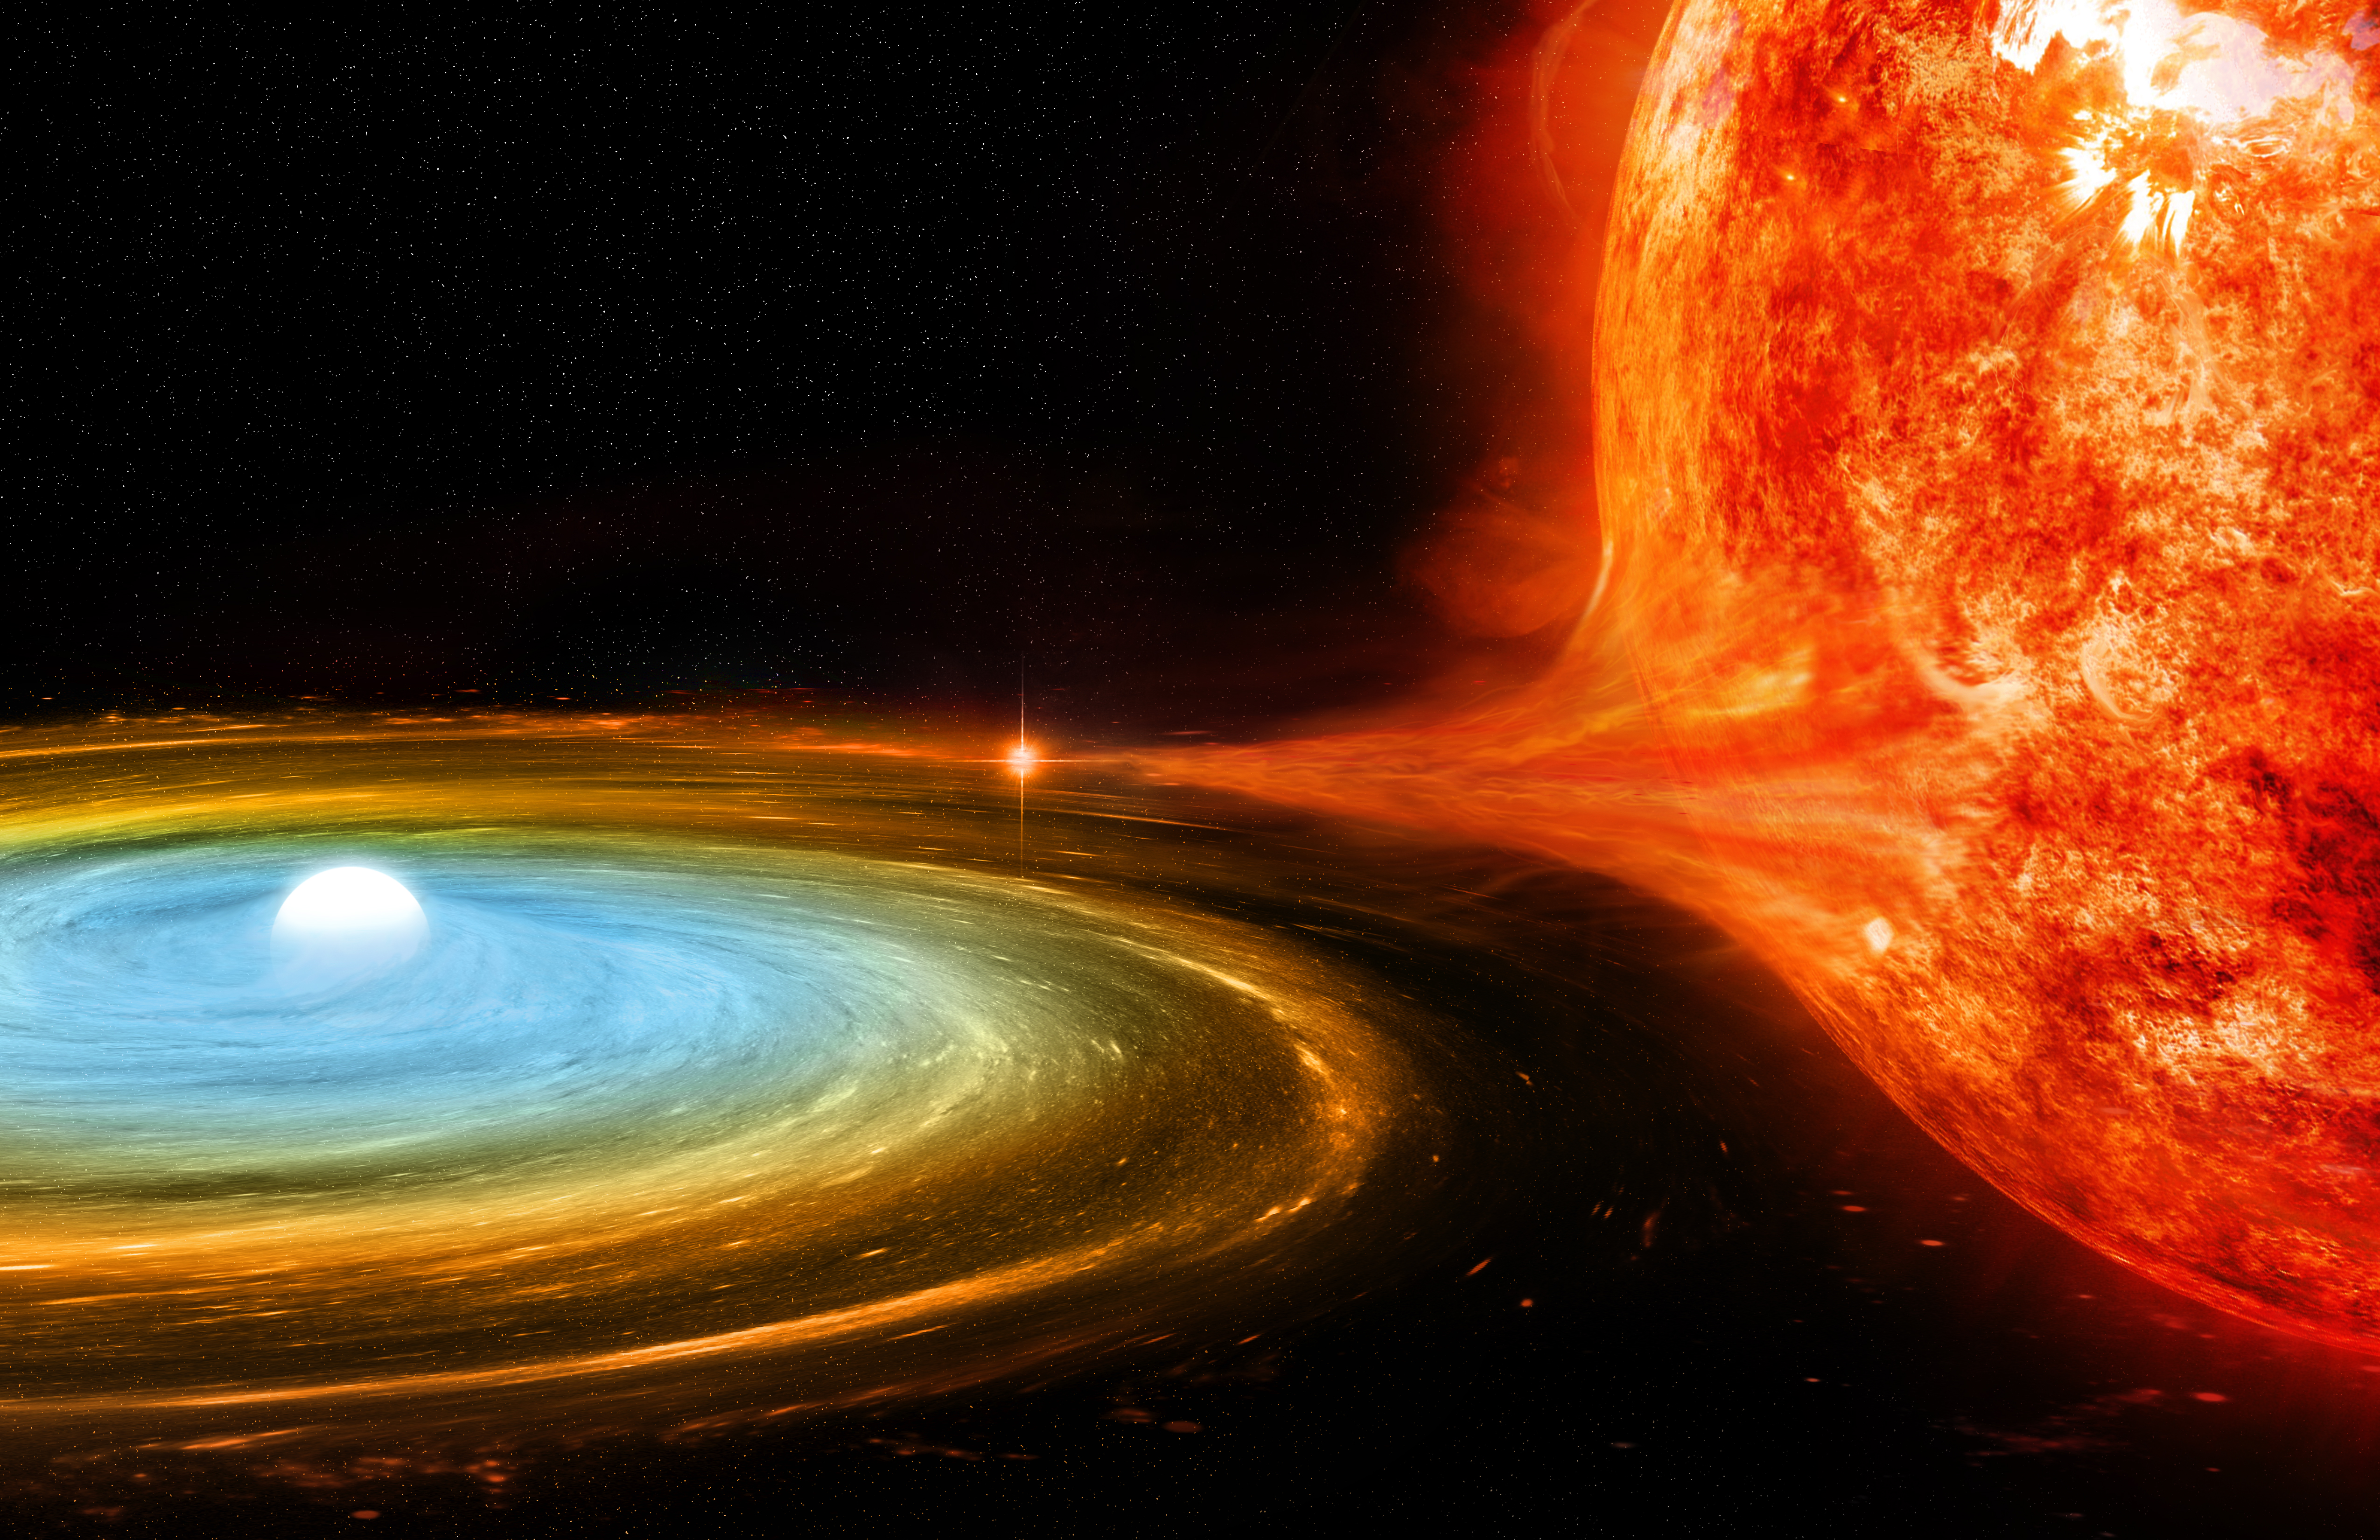
\includegraphics[width=0.88\linewidth,height=0.48\textheight,keepaspectratio]{../figs/source/en/fig-05-01.jpg}

% DOCX paragraph 479
\caption{\emph{Representación artística de la acreción de materia en Sco X-1. La estrella de neutrones arranca materia de su compañera, que es de mayor tamaño pero tiene una masa inferior. La materia robada de esta manera forma un disco de acreción que vierte materia lentamente sobre la estrella de neutrones. © NASA/CXC/M. Weiss.}}\label{fig:05-01}
\end{figure}

% DOCX paragraph 481
Pero algo fallaba en este escenario, por lo demás muy razonable. Para producir una radiación tan intensa es necesario que, en la transferencia de una estrella a otra, la materia experimente un tremendo salto gravitatorio, mucho mayor de lo que cabría esperar si nos basamos en las dimensiones que suponemos que tienen las dos estrellas.

% DOCX paragraph 482
Para entender mejor este fenómeno, intentemos pensar en una central hidroeléctrica o en un molino de agua. Ambas estructuras funcionan de acuerdo con el mismo principio físico: la conversión\index{energia@energía!conversión} de energía de una forma, la \emph{potencial\index{energia@energía!potencial (gravitatoria)}}, a otra, la \emph{cinética\index{energia@energía!cinética}}. En otras palabras, cuando se toma agua de una posición elevada, su caída se aprovecha para realizar trabajo: hacer funcionar las turbinas que producen electricidad o mover la rueda que muele el grano y lo transforma en harina. El agua puede caer desde cientos de metros o desde unos pocos, lo cual claramente influye en la cantidad de trabajo que se genera. Expresándolo con más precisión: estamos convirtiendo la \emph{energía potencial gravitatoria} en energía cinética. La energía potencial gravitatoria es la energía que tiene un objeto (en este caso, el agua) por el hecho de encontrarse en un campo gravitatorio y que puede liberar si se deja caer, transformándola en \emph{energía cinética}; esta es la energía que un objeto posee por estar en movimiento a una determinada velocidad (un objeto en reposo tiene energía cinética igual a cero).

% DOCX paragraph 483
Esencialmente, es la misma conversión que se piensa que ocurre en el caso de Sco X-1\index{Scorpius X-1 (Sco X-1)}: la materia sustraída a la estrella secundaria (que representa el agua en nuestro ejemplo) habría adquirido una cierta cantidad de energía cinética en la caída hacia la primaria, más masiva pero también más compacta. Por último, en el momento de la colisión entre la materia y la superficie, la energía cinética habría experimentado una transformación adicional. En lugar de convertirse en energía eléctrica, como en el caso de la central hidroeléctrica, habría producido radiación\index{rayos X!radiación} electromagnética en la banda de rayos X.

% DOCX paragraph 484
Sin embargo, como anticipábamos, algo fallaba en este panorama. A juzgar por la energía producida, el salto gravitatorio que experimentaba la materia arrancada de la estrella secundaria antes de caer sobre la superficie tenía que haber sido enorme, mucho mayor de lo que se habría esperado si la primaria hubiera sido una estrella corriente de 1,4 masas solares. Volviendo al ejemplo de la central hidroeléctrica, era como si el agua estuviera cayendo de una montaña casi un millón de veces más alta de lo que se había supuesto para impulsar la turbina situada más abajo. En resumen, la evidente discrepancia entre las expectativas teóricas y las observaciones indicaba con bastante claridad que algo fallaba en el enfoque teórico y, en particular, en el tipo de estrella que podía ser la primaria.

% DOCX paragraph 485
Otro dato de observación contribuyó a que el panorama resultara aún más enigmático: la fuente de rayos X\index{rayos X!radiación} también era sumamente \emph{variable}. En esencia, la luminosidad de Sco X-1\index{Scorpius X-1 (Sco X-1)} mostraba variaciones significativas a lo largo del tiempo, con diferencias de un 10 o un 20 por ciento en escalas de tiempo de minutos o incluso decenas de segundos, mucho más cortas de lo que se esperaba para una estrella corriente de 1,4 masas solares.\textsuperscript{\hyperlink{note:05-04}{4}}

% DOCX paragraph 486
El golpe de gracia en esta situación decididamente confusa y desorientadora vino con el descubrimiento (en 1964) de otra fuente X muy luminosa, que recibió el nombre de Cygnus X-1 (o simplemente Cyg X-1\index{Cyg X-1}). Como puedes adivinar, era la primera fuente en la banda de rayos X\index{rayos X!radiación} en el interior de la constelación de Cygnus, el Cisne.

% DOCX paragraph 487
De nuevo, se trataba de un sistema binario, pero las masas en cuestión eran bastante mayores: la primaria se estimó en 40 masas solares y la secundaria en 15 (de ahí que se le diera el nombre de \emph{binaria de rayos X\index{rayos X!radiación} de alta masa}, o HMXB\index{HMXB (binaria de rayos X de alta masa)}). En cualquier caso, la luminosidad en la banda X de Cyg X-1 también era muy alta, tanto que resultaba anómala. Además, igual que en el caso de Sco X-1\index{Scorpius X-1 (Sco X-1)}, el sistema binario de Cyg X-1 también tenía un periodo\index{orbita@órbita!periodo} orbital breve (aproximadamente 5,6 días), y esto permitió a los astrónomos ver la emisión en la banda óptica de la primaria, una estrella de la que se sabía que era masiva y luminosa, pero por lo demás relativamente corriente.\textsuperscript{\hyperlink{note:05-03}{3}} En la figura \ref{fig:05-02} aparece una imagen de Cyg X-1 en la banda de rayos X, que nos permite apreciar lo difícil que es conseguir una imagen de buena resolución en esta banda.

% DOCX paragraph 488
Una vez más, sin embargo, lo que hacía de Cyg X-1\index{Cyg X-1} algo realmente misterioso era su variabilidad\index{variabilidad}: podía bajar de un segundo e incluso llegar al orden de unos pocos milisegundos. Como hemos visto, un tiempo de variabilidad tan corto implicaba unas dimensiones muy pequeñas, muy por debajo de los 300 kilómetros de radio. En aquellos años no se conocía ningún modelo que explicara cómo una estrella tan pequeña podía producir una emisión como esta en la banda X.\textsuperscript{\hyperlink{note:05-04}{4}}

% DOCX paragraph 491
\begin{figure}[htbp]
\centering
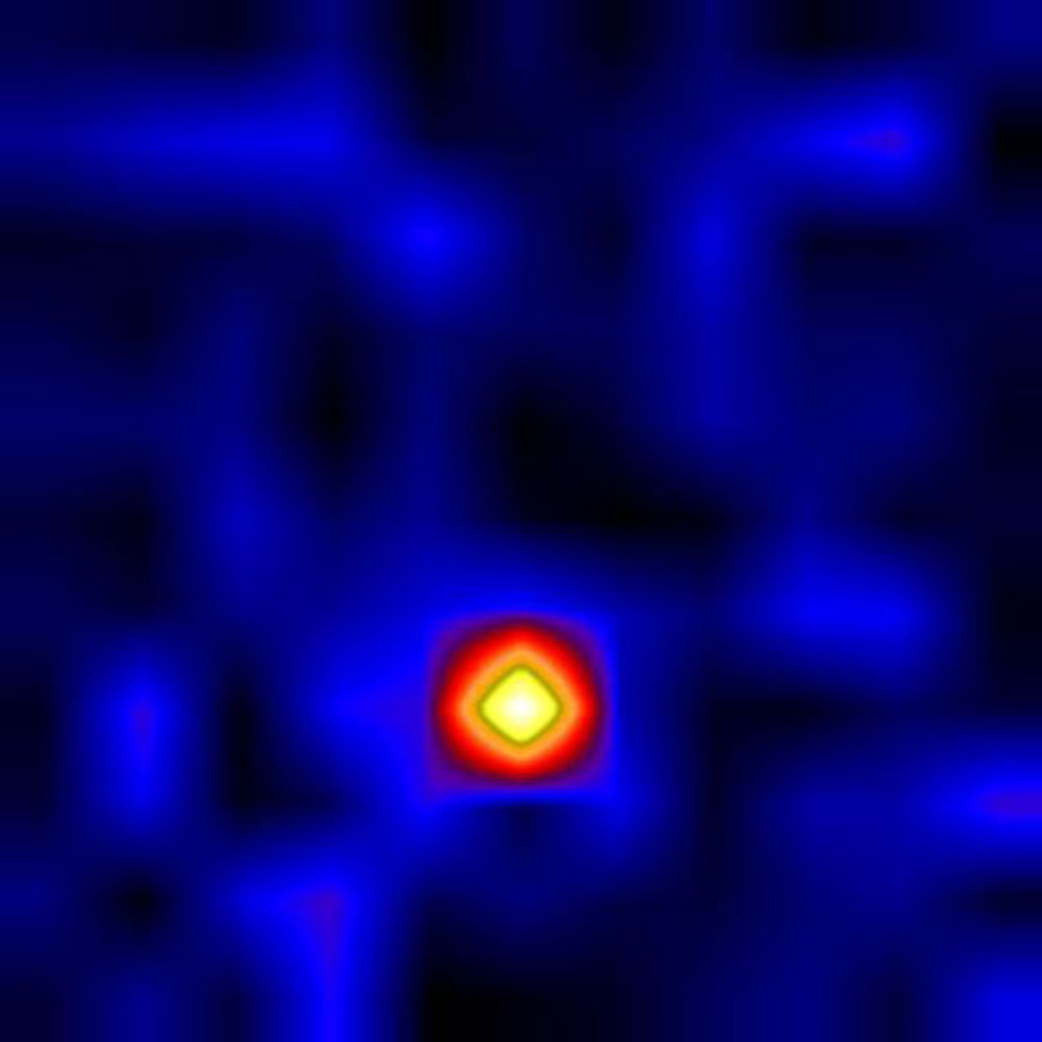
\includegraphics[width=0.88\linewidth,height=0.48\textheight,keepaspectratio]{../figs/pdf/en/fig-05-02.pdf}

% DOCX paragraph 493
\caption{\emph{Imagen de Cyg X-1 en la banda de rayos X. La emisión está vinculada a un disco de acreción que extrae materia de una estrella de 40 masas solares y la vierte sobre un agujero negro de 15 masas solares. © NASA/Marshall Space Flight Center.}}\label{fig:05-02}
\end{figure}

% DOCX paragraph 495
En resumen, los astrónomos de principios de la década de 1960 se encontraban ante un rompecabezas difícil de resolver. Las observaciones de Sco X-1\index{Scorpius X-1 (Sco X-1)} y Cyg X-1\index{Cyg X-1} demolieron muchas de las certidumbres que la astrofísica nuclear había tardado unos treinta años en construir. No cabía duda: las observaciones revelaban fuentes de tamaño muy pequeño (diminutas a cualquier «escala astronómica») y, al mismo tiempo, extremadamente masivas (es decir, con una masa muy grande), que producían enormes cantidades de radiación de alta energía\index{energia@energía!eficiencia de producción} (sobre todo en la banda X). La astrofísica estelar no podía explicar su naturaleza y la física nuclear no conocía ningún mecanismo capaz de arrojar luz sobre su enorme eficiencia en la producción de energía. Al mismo tiempo, sin embargo, Sco X-1\index{Scorpius X-1 (Sco X-1)} y Cyg X-1 también representaban una oportunidad increíble: ¡no hay nada más interesante para un científico que descubrir algo aparentemente inexplicable!

% DOCX paragraph 496
Pronto quedó claro que el enigma de las dos fuentes no tenía solución a menos que se considerara la extraña teoría de la gravedad propuesta casi cincuenta años antes por el físico alemán Albert Einstein. Una teoría que predecía la existencia de objetos extremadamente pequeños capaces de generar una gran curvatura del espaciotiempo.

% DOCX paragraph 497
En el resto de este capítulo aprenderemos lo que sabemos hoy sobre esa maravilla de la naturaleza responsable de la emisión de Sco X-1\index{Scorpius X-1 (Sco X-1)}.

% DOCX paragraph 500
\section{Lo que queda de una estrella masiva}\label{sec:05-remnant}

% DOCX paragraph 502
Como ocurre de manera casi sistemática en astrofísica, no tardó en florecer una multitud de teorías y escenarios que intentaban explicar las observaciones de Sco X-1\index{Scorpius X-1 (Sco X-1)} y Cyg X-1\index{Cyg X-1}. La mayoría de estas hipótesis resultaron estar lejos de la realidad, aunque todas eran físicamente correctas. Se trata de un fenómeno bastante común en un campo científico como la astrofísica, en el que debemos deducir los mecanismos físicos de funcionamiento a través de simples observaciones, sin poder crear un dispositivo experimental para poner a prueba esta o aquella hipótesis. Volveremos a este tema al final del capítulo 6.

% DOCX paragraph 503
El primero que propuso el modelo que actualmente se considera que explica correctamente los fenómenos relacionados con Sco X-1\index{Scorpius X-1 (Sco X-1)} fue el astrofísico soviético Iosif Shklovsky\index{Shklovsky, Iosif}, quien, en febrero de 1967, concluyó que ninguno de los supuestos previos era satisfactorio; todos tenían aspectos que parecían poco realistas o insuficientes para dar cuenta de las observaciones. No obstante, estaba convencido de que había un enfoque bastante sencillo para explicar la fenomenología de Sco X-1\index{Scorpius X-1 (Sco X-1)}: su modelo requería la formación de un disco de acreción\index{disco de acreción} que, partiendo de la estrella secundaria, hiciera caer materia sobre un objeto extremadamente compacto, es decir, una \emph{estrella de neutrones\index{estrella de neutrones}}.\textsuperscript{\hyperlink{note:05-05}{5}}

% DOCX paragraph 504
Lo que siempre me ha sorprendido de la hipótesis ---correcta--- que presentó Shklovsky es que en aquella época ¡nadie había observado jamás una estrella de neutrones! Desde la década de 1930, tras el descubrimiento del neutrón, se creía teóricamente posible la existencia de un objeto estelar compuesto solo de esas partículas elementales eléctricamente neutras, y eso era todo. Walter Baade\index{Baade, Walter} y Fritz Zwicky\index{Zwicky, Fritz} propusieron esta idea en un artículo que resultó ser uno de los más visionarios de la astrofísica: trataba conceptos como la explosión de supernova\index{supernova} (que veremos seguidamente), la estrella de neutrones y el origen de los rayos cósmicos.\textsuperscript{\hyperlink{note:05-06}{6}} La idea de una estrella de neutrones propuesta por Baade y Zwicky no formaba parte, desde luego, de una teoría desarrollada de manera sistemática. De hecho, apareció literalmente en una nota a pie de página del artículo de 1934. Pero en 1967 eso fue suficiente para cambiar la forma de entender Sco X-1\index{Scorpius X-1 (Sco X-1)} y dejar de lado otras interpretaciones fascinantes pero incorrectas.

% DOCX paragraph 505
El modelo de Shklovsky ofrecía una explicación sencilla de lo que emergía de las observaciones, si bien a costa de introducir en su receta un «ingrediente exótico»: un objeto compacto esquivo cuya existencia y origen eran plausibles desde el punto de vista de la astrofísica (se sabía que las estrellas masivas podían explotar y quizá dejar un residuo), pero que nadie había identificado antes. Quedaba pues un margen de incertidumbre, que se desvaneció a finales de ese mismo año. En Cambridge, la estudiante británica Jocelyn Bell\index{Bell, Jocelyn} y su director Antony Hewish\index{Hewish, Antony} identificaron un objeto astronómico capaz de generar una emisión de radio pulsada y regular: el primer descubrimiento de una estrella de neutrones.\textsuperscript{\hyperlink{note:05-07}{7}}

% DOCX paragraph 506
Ahora bien, ¿qué es una estrella de neutrones y cómo se forma? Para responder a esta pregunta tenemos que volver a lo que vimos al principio del capítulo, cuando recordé que una estrella produce energía mediante una serie de procesos de fusión termonuclear\index{fusion termonuclear@fusión termonuclear} de elementos con \emph{masa\index{atomico@atómico!masa} atómica} creciente.\textsuperscript{\hyperlink{note:05-08}{8}} El hidrógeno se fusiona para formar helio, el helio para formar carbono, el carbono para formar neón, y así sucesivamente. Un aspecto esencial para que este fenómeno tenga éxito es que se produzca una cierta cantidad de energía cada vez que ocurre. La cantidad de energía liberada depende de los elementos que intervienen en la fusión: como si subiera por una escalera, la energía liberada aumenta al ritmo de su masa atómica. Así pues, la transformación de hidrógeno en helio produce menos energía que el paso siguiente: de helio a carbono. Y lo que es más importante, cada una de estas fusiones libera energía en forma de calor, y por esa razón todas se llaman \emph{reacciones termonucleares exotérmicas\index{reacciones termonucleares!exotérmicas}}.

% DOCX paragraph 507
Sin embargo, esta escala tiene inevitablemente un límite superior, a partir del cual ya no se puede producir energía. El hierro representa ese límite, en particular su isótopo con masa atómica 56 (que se escribe \textsuperscript{56}Fe). En consecuencia, la fusión de dos de sus átomos requiere más energía de la que libera, porque es necesario suministrar al sistema la energía suficiente para juntar los átomos y fusionarlos. Las fusiones de este tipo, que absorben energía del exterior en forma de calor, se llaman \emph{reacciones termonucleares endotérmicas\index{reacciones termonucleares!endotérmicas}}.

% DOCX paragraph 508
No todas las estrellas alcanzan a lo largo de su vida el punto más alto de esta escalera; de hecho, la mayoría (es decir, las que están por debajo de una docena de masas solares) se detienen mucho antes. La razón es muy sencilla: para desarrollarse, los procesos de fusión necesitan temperaturas y densidades críticas, por debajo de las cuales no se desencadenan. Esto se debe a que, en general, los átomos que participan en estas reacciones tienen una carga eléctrica positiva. Por tanto, es necesario que se alcancen temperaturas y densidades suficientemente elevadas para superar el empuje repulsivo que tendería a hacer que dos átomos con igual carga se separasen. Por otra parte, cuanto mayor es la masa de una estrella, más altas son la densidad y la temperatura en su interior. Así, las estrellas «ligeras» (con poca masa) solo queman elementos ligeros, mientras que las estrellas «pesadas» (con mucha masa) pueden quemar tanto elementos ligeros como pesados; es decir, átomos con un gran número de protones y neutrones, como el neón y el silicio. En particular, las estrellas del orden de 20 o 30 masas solares tienen suficiente masa para alcanzar temperaturas internas capaces de desencadenar reacciones en las que intervienen los elementos más pesados y, por tanto, pueden subir la escalera hasta el hierro.

% DOCX paragraph 509
Dado que la temperatura y la densidad aumentan a medida que bajamos hacia el centro de la estrella, los elementos más pesados se producen en sus regiones más interiores. A la inversa, los más ligeros se forman en las zonas más externas. A lo largo de su vida, una estrella masiva desarrolla una estructura parecida a la de una cebolla: en las capas exteriores abundan los elementos ligeros, mientras que las capas interiores son ricas en elementos pesados. Si la estrella tiene bastante masa, su núcleo estará compuesto de hierro\index{hierro} producido por la fusión de elementos más pesados, como el neón, el oxígeno y el silicio.

% DOCX paragraph 510
Cuando se ha agotado todo el combustible que se puede convertir en hierro, la estrella se encuentra en un punto de inflexión fundamental, porque la fusión que da lugar a elementos más pesados absorbería energía en vez de producirla. A partir de ahí, ya nada será igual. Como puedes imaginar, la imposibilidad de generar más energía compromete el equilibrio que se había mantenido hasta ese momento. Durante millones de años, fueron justamente los procesos de fusión nuclear los que liberaron la energía necesaria para resistir la fuerza de la gravedad, que de otro modo haría que la estrella sufriera una implosión.

% DOCX paragraph 511
Llegados a este punto, una analogía nos puede ayudar una vez más a comprender lo que sucede. Imaginemos que una estrella es como un globo aerostático, bien hinchado con aire caliente gracias al chorro de un potente quemador. Desde el punto de vista de la física, el globo se mantiene tenso porque la presión\index{presión!interna} de su interior es más elevada que la de fuera. La liberación de energía que se produce cuando el quemador consume su combustible es la fuente de esa presión. En una estrella, en cambio, lo que genera la presión es la energía que liberan las reacciones nucleares. Cuando la presión interior ya no está disponible porque el quemador se ha quedado sin combustible, el globo, vencido por la presión externa\index{presión!externa} y la gravedad, simplemente se desinflará. La estrella, por otra parte, una vez agotado el combustible y sin poder producir más hierro, sufrirá una implosión bajo su propio \emph{peso gravitatorio}, colapsando hacia el centro.

% DOCX paragraph 512
Cuando esto sucede en una estrella de 20 o 30 masas solares, el núcleo\index{hierro!núcleo} está compuesto en su totalidad de hierro\index{hierro} y tiene un radio de unos 10\,000 kilómetros. Incapaz de soportar su propio peso y privado del sostén de la presión\index{degeneración!presión}, el núcleo de hierro se contrae rápidamente y se precipita en caída libre hacia el centro, igual que le pasaría a un globo aerostático. Durante esta fase, la materia del núcleo estelar sigue comprimiéndose, alcanzando temperaturas y, sobre todo, densidades extremas. La implosión continúa hasta que la densidad del núcleo estelar llega a ser tal que «empaqueta» los átomos en un volumen muy pequeño, aplastándolos unos contra otros. En este punto se desarrolla una presión nueva, increíble, cuyo origen no está en la termodinámica (es decir, vinculado al hecho de que la temperatura debe subir si la densidad sube), sino en la mecánica cuántica\index{mecánica cuántica}. Los átomos presentes en el núcleo de hierro en caída libre están tan comprimidos que las reglas de la mecánica cuántica (según las cuales partículas como los neutrones no pueden estar demasiado cerca unas de otras) dan lugar a la llamada \emph{presión de degeneración}, que repentinamente se opone a la contracción.\textsuperscript{\hyperlink{note:05-09}{9}}

% DOCX paragraph 513
Esta nueva y enorme presión\index{degeneración!presión} es capaz de detener el colapso\index{gravitatorio!colapso}\index{colapso|see{gravitatorio, colapso}} gravitatorio del núcleo de hierro, que ahora ha alcanzado un radio de solo 100 kilómetros y una temperatura de miles de millones de kelvin. Ya no es posible contraerse más allá de ese núcleo incandescente, cuya materia es la más densa y rígida que conocemos. Mientras tanto, sin embargo, el resto de la estrella sigue cayendo, «sin darse cuenta» de que la contracción del núcleo se ha detenido: tan solo la parte más interior está sometida a la presión\index{degeneración!presión} de degeneración, lo cual crea las condiciones apropiadas para una espectacular onda de choque\index{choque}. En un momento dado, al no poder seguir avanzando, el manto estelar «rebota» en la superficie del núcleo de hierro, generando un enorme \emph{frente de choque} que se desplaza hacia fuera desde el corazón de la estrella a velocidad supersónica. El frente de choque, saturado ya de la energía potencial gravitatoria adquirida durante la caída del manto, se ve «empujado» aún más hacia fuera por la energía de los neutrino\index{neutrino}s emitidos en grandes cantidades desde el núcleo caliente y denso. El resultado es catastrófico y espectacular al mismo tiempo: la onda de choque consigue atravesar la estrella entera, barriendo a enormes velocidades toda la materia con la que se encuentra. En unas pocas decenas de segundos, una estrella de 20 o 30 masas solares queda pulverizada por una tremenda explosión, una \emph{supernova\index{estrella de neutrones!supernova}\index{supernova}}. Así pues, una explosión de supernova no es más que el fenómeno producido por la parte central de una estrella que «rebota» al golpear el núcleo duro creado por la presión de degeneración.

% DOCX paragraph 514
Mientras las capas externas de la estrella salen despedidas, una enorme cantidad de radiación en la banda visible acompaña la explosión, gracias a lo cual el proceso puede detectarse incluso a grandes distancias. Si el fenómeno se diera cerca de nosotros (por ejemplo, dentro de nuestra galaxia), lo podríamos ver a simple vista, ¡incluso a plena luz del día! Eso es justamente lo que ocurrió en 1054, cuando unos astrónomos chinos registraron la presencia de una nueva estrella en el cielo diurno. Ahora sabemos que se trataba de una supernova\index{supernova} en la constelación\index{Cangrejo!constelación} del Cangrejo. En la actualidad, las observaciones astronómicas nos permiten estudiar los «restos» de explosiones de este tipo en lo que los astrónomos llaman \emph{nebulosa\index{nebulosa}s}. Están compuestas de los residuos filamentosos de toda la materia estelar que la explosión ha dispersado, proyectándola a una velocidad enorme, del orden de 1500 kilómetros por segundo, en volúmenes astronómicos de 10 años luz. Como comparación, el tamaño del sistema solar es de tan solo cinco horas luz.

% DOCX paragraph 515
En la figura \ref{fig:05-03} se puede ver una imagen muy bonita de la nebulosa del Cangrejo, que de hecho es una superposición de dos imágenes tomadas con filtros diferentes para destacar los diversos componentes de su emisión. Observa que esta técnica nos permite apreciar claramente la presencia de numerosos filamentos que emanan del centro de la nebulosa y son el resultado de la explosión de la supernova. ¡Eso es lo que queda de la estrella que ha explotado! Justo en el centro de esta nebulosa hay una diminuta estrella de neutrones que, como pronto veremos, es simplemente un condensado de extremos.

% DOCX paragraph 517
\begin{figure}[htbp]
\centering
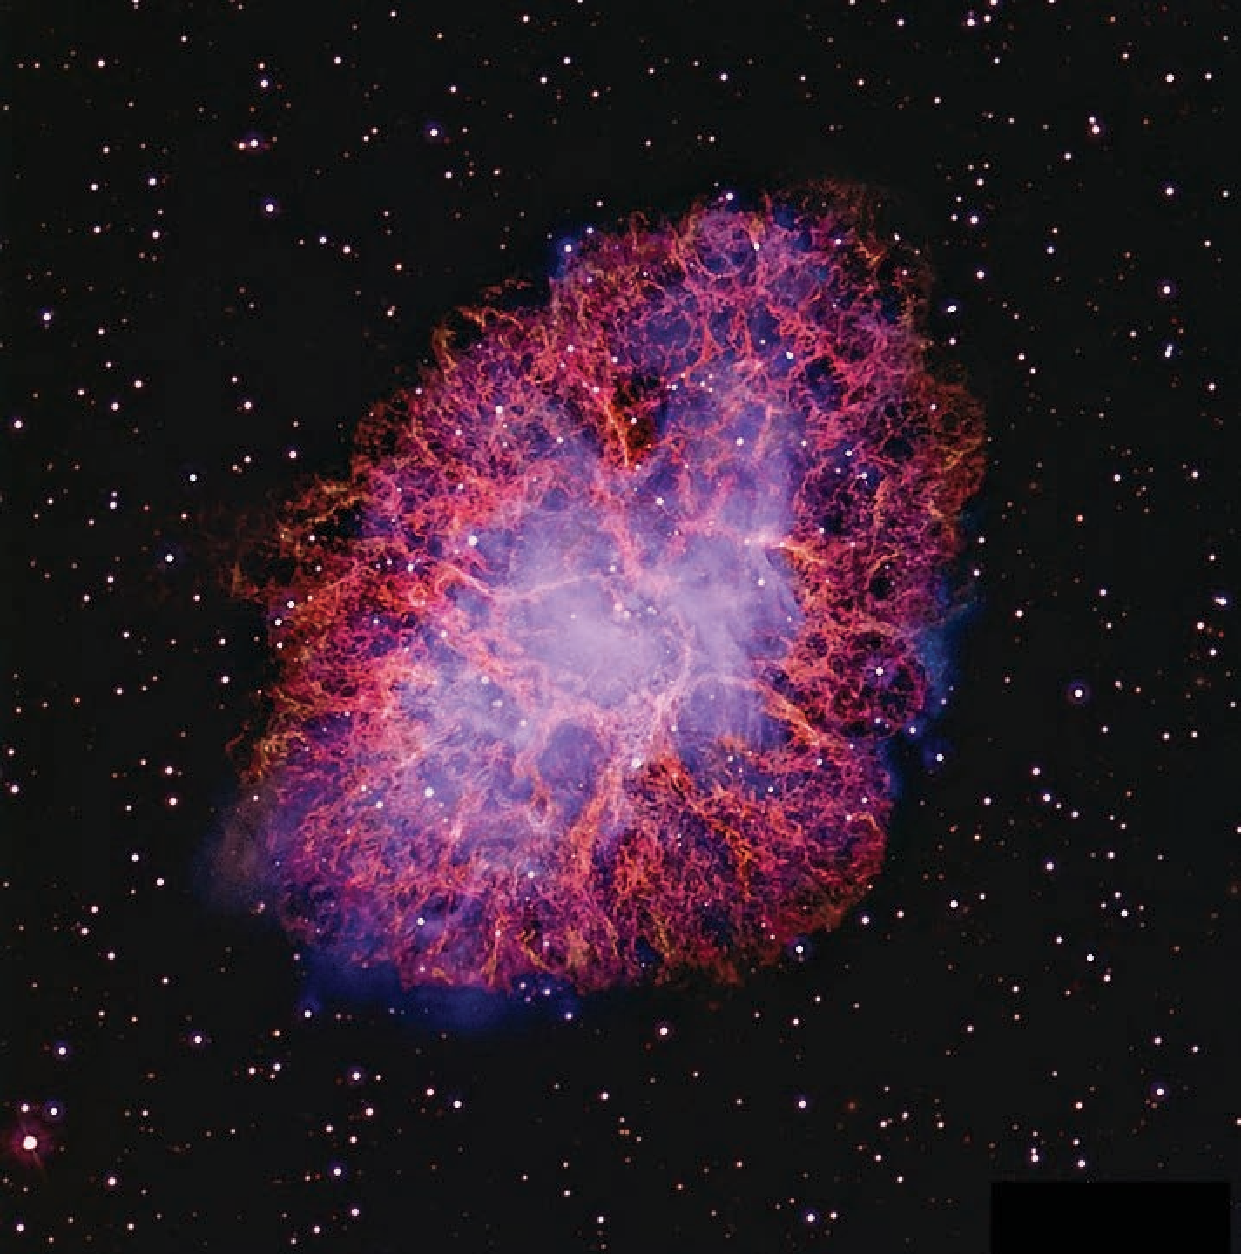
\includegraphics[width=0.88\linewidth,height=0.48\textheight,keepaspectratio]{../figs/pdf/en/fig-05-03.pdf}

% DOCX paragraph 519
\caption{\emph{Superposición de diferentes imágenes en la parte visible del espectro de la «nebulosa del Cangrejo», los restos de la explosión de supernova que tuvo lugar en 1054 en la constelación de Cáncer. © The Liverpool Telescope.}}\label{fig:05-03}
\end{figure}

% DOCX paragraph 521
Las explosiones de supernova\index{supernova} son muy comunes en astrofísica, y las estimaciones muestran que, tan solo en nuestra galaxia, la Vía Láctea\index{Vía Láctea}, se puede observar una supernova más o menos cada 30 o 40 años. La última, SN1987A\index{SN1987A}, se hizo visible en 1987, hace más de 30 años, y los astrónomos esperan ansiosos la próxima… No cabe duda de que será un espectáculo memorable, que observaremos de muchas maneras diferentes, como explicaré enseguida.

% DOCX paragraph 525
\section{Un condensado de extremos}\label{sec:05-extremes}

% DOCX paragraph 527
Volvamos a Sco X-1\index{Scorpius X-1 (Sco X-1)} y a aquello de lo que más queremos hablar en este libro: la gravedad. Hay un objeto vinculado a una de las expresiones más extremas de la física y, en particular, de la gravedad, cuya aparición acompaña los increíbles fuegos artificiales que genera una explosión de supernova\index{supernova}.

% DOCX paragraph 528
Casi invisible en el centro de una nebulosa\index{nebulosa} se esconde el núcleo de la estrella que explotó y que sobrevivió a su colapso\index{gravitatorio!colapso}, un cuerpo celeste extremadamente denso y compacto cuyas propiedades solo pueden provocar asombro. Personalmente, siempre me ha impresionado que el acto final de la vida luminosa y ajetreada de una estrella masiva (así como el proceso catastrófico que revela su muerte) señale también el nacimiento de uno de los objetos más fascinantes de la física: una estrella de neutrones. Es un objeto cuyo radio alcanza unos doce kilómetros, pero que concentra una masa mucho mayor que la del Sol (se han observado ejemplos de estrellas de neutrones con dos masas solares).

% DOCX paragraph 529
Así pues, intenta visualizar un cuerpo celeste del tamaño de la parte central de una gran ciudad como Londres o Nueva York, pero cuya masa es enorme y cuya densidad es inimaginable para nuestro sentido de las escalas físicas. De forma esquemática y explicativa, este llamativo contraste se muestra en la figura \ref{fig:05-04}, donde se comparan las dimensiones típicas de una estrella de neutrones (con un radio estimado de entre 12 y 14 kilómetros) y las de la parte interior de Londres, delimitada por las circunvalaciones norte y sur. El río Támesis atraviesa la ciudad de oeste a este y, más allá, se puede ver el anillo de la autopista M25…

% DOCX paragraph 531
\begin{figure}[htbp]
\centering
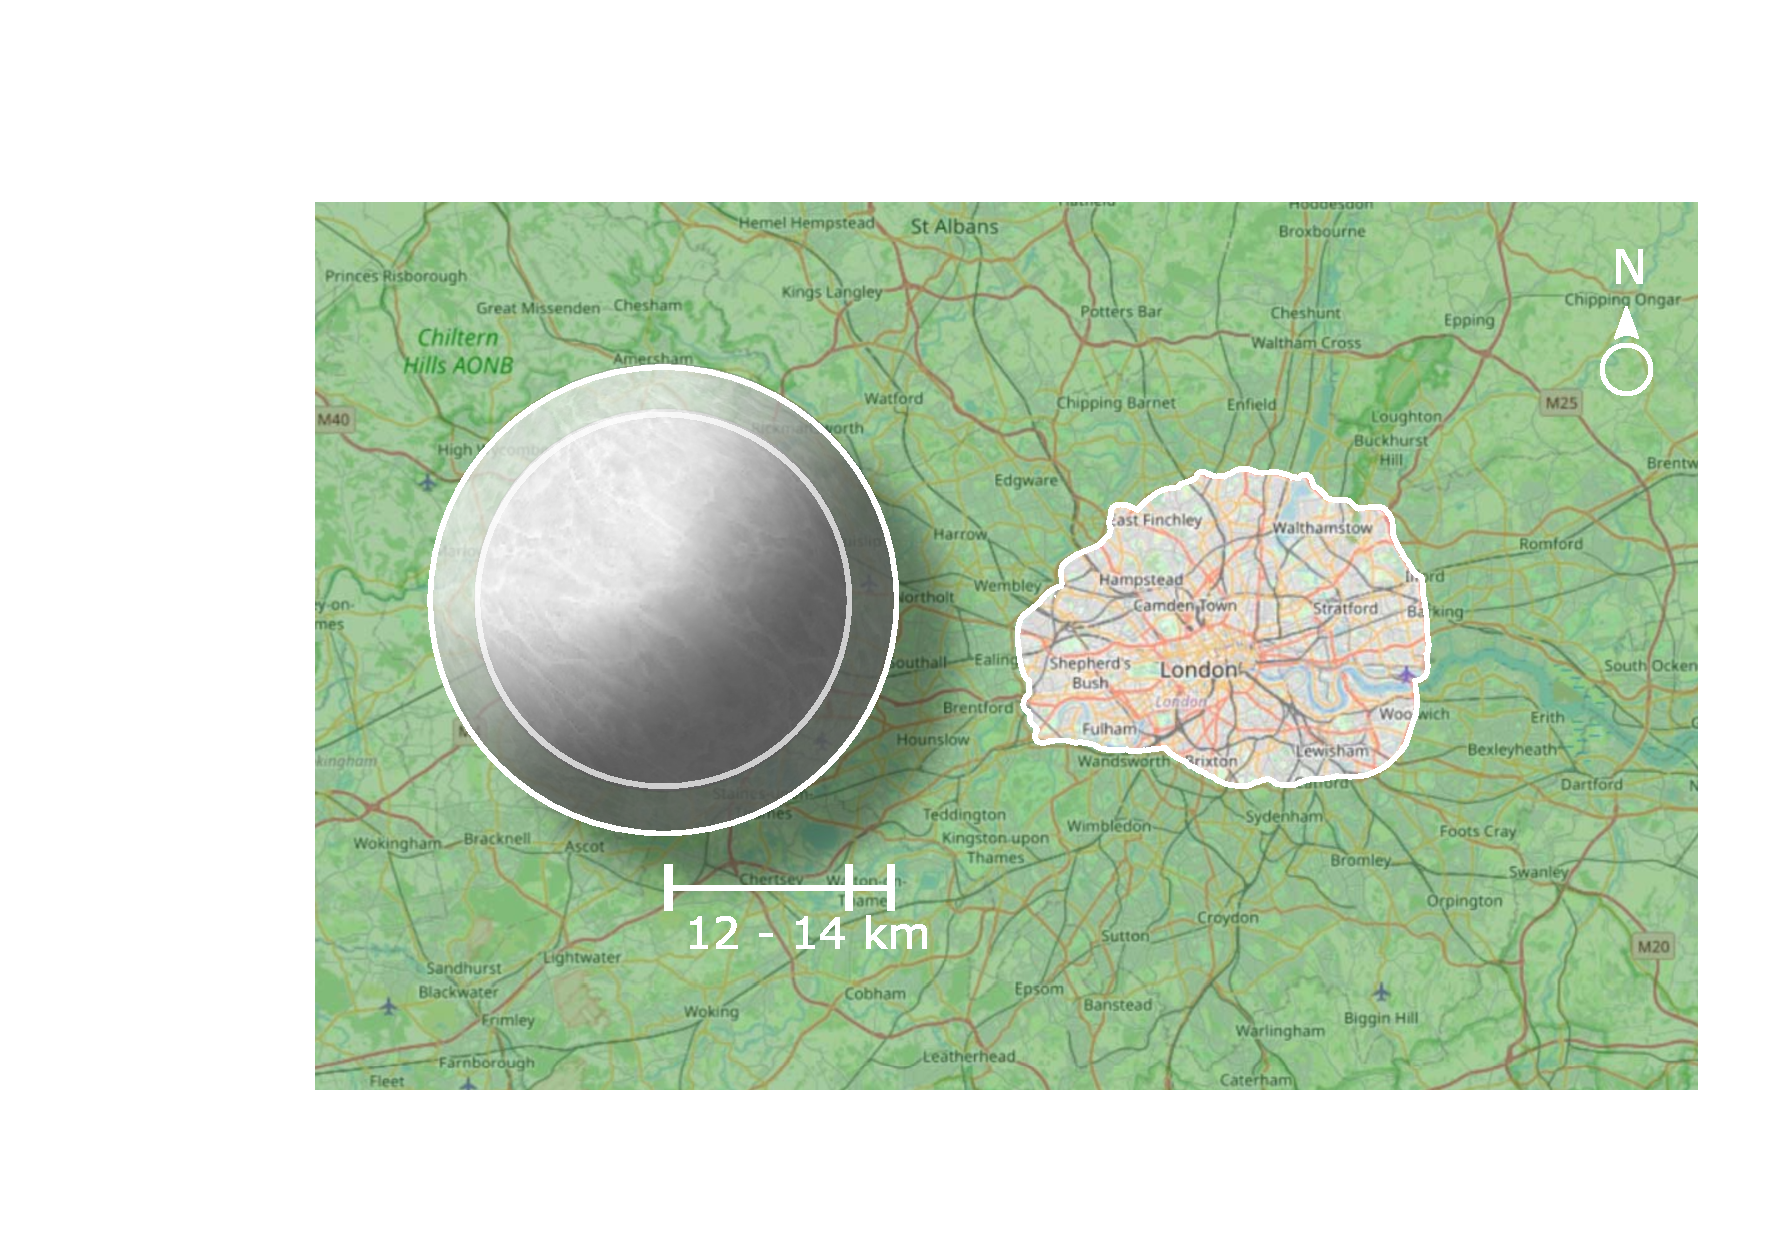
\includegraphics[width=0.88\linewidth,height=0.48\textheight,keepaspectratio,trim=149bp 72bp 41bp 96bp,clip]{../figs/pdf/en/fig-05-04.pdf}

% DOCX paragraph 533
\caption{\emph{La ilustración compara las dimensiones típicas de una estrella de neutrones y las de la parte interior de Londres, delimitada por las circunvalaciones norte y sur. © L. Weih / LR / mapa © colaboradores de OpenStreetMap (CC-BY-SA 2.0) / R. K. Lazenby.}}\label{fig:05-04}
\end{figure}

% DOCX paragraph 535
Durante este viaje hemos insistido varias veces en que nuestro sentido de la realidad y de la escala física está necesariamente determinado por nuestras experiencias en este planeta. Por tanto, nos resulta difícil siquiera imaginar las condiciones físicas asociadas a una estrella de neutrones típica. Pero podemos intentarlo, empezando por su densidad\index{estrella de neutrones!densidad} (es decir, cuánta materia se concentra en un volumen dado). Para referirnos a una densidad que a todos nos resulta familiar, consideremos el agua: un gramo por centímetro cúbico, o bien 1 g/cm\textsuperscript{3}. La densidad media de las rocas es bastante similar: 2,6 g/cm\textsuperscript{3}, por tanto, unas dos veces la del agua. Pues bien, la densidad media de una estrella de neutrones es aproximadamente 10\textsuperscript{14} g/cm\textsuperscript{3} y, en el centro, puede alcanzar los 10\textsuperscript{15} g/cm\textsuperscript{3}. En otras palabras, estamos hablando de densidades que son mil billones de veces la del agua. Si quieres una comparación todavía más directa, intenta imaginar un único centímetro cúbico de material procedente de una estrella de neutrones ---o sea, una cantidad como la de un terrón de azúcar--- que contenga una masa igual a la de toda la cordillera de los Alpes, desde los Ligures hasta los Friulanos. Advertencia: aquí no me refiero al peso, aunque la analogía seguiría siendo correcta, sino al número de átomos (en realidad, protones, neutrones y electrones) contenidos en nuestro cubito de estrella de neutrones. Si los contáramos de uno en uno, descubriríamos que su número es comparable al de los átomos de la cordillera.

% DOCX paragraph 536
Está claro que estas densidades son inimaginables para nosotros; se alcanzan cuando todas las partículas elementales están comprimidas unas contra otras y las funciones de onda que las describen casi se superponen.\textsuperscript{\hyperlink{note:05-10}{10}} Para entender mejor este concepto, piensa en un átomo en condiciones normales (las que se dan en la materia de la que estamos hechos tú y yo) como si fuera una bola de algodón de azúcar, compuesta en su mayor parte de aire y filamentos de azúcar alejados entre sí. En esta analogía, el algodón de azúcar representa la \emph{nube\index{electron@electrón!nube} electrónica}, es decir, el volumen ocupado por los electrones (o, mejor dicho, por sus funciones de onda) que giran vertiginosamente alrededor del núcleo. Hay algo muy denso y pesado en el centro del algodón de azúcar, parecido a uno de esos pequeños plomos que se usan para pescar: el núcleo del átomo. Para comprender las dimensiones relativas y el hecho de que un átomo está esencialmente «vacío», imagina que la nube de algodón de azúcar es aproximadamente 100\,000 veces mayor que el núcleo, un punto diminuto pero mucho más «pesado» que todo el resto. Así, partiendo de esta imagen, podemos imaginar que, en los átomos que componen una estrella de neutrones, las nubes de algodón de azúcar (es decir, las nubes electrónicas) prácticamente desaparecen y solo quedan los pequeños puntos de su centro. Además, estos puntos están empaquetados unos encima de otros a densidades más extremas que en una lata de sardinas. Los electrones siguen presentes en esta enorme aglomeración de núcleos, pero están obligados a moverse en espacios muy pequeños y no pueden crear las nubes suaves que crearían en condiciones normales.

% DOCX paragraph 537
Estaría muy bien, y sería muy interesante, reproducir estas condiciones físicas de densidad extrema en un experimento de laboratorio, para comprender mediante mediciones directas cómo es posible comprimir hasta ese punto las funciones de onda que describen las partículas elementales en el centro del núcleo atómico. Lamentablemente, como veremos mejor más adelante, eso no es posible: las densidades que somos capaces de reproducir en el laboratorio, incluso haciendo chocar entre sí núcleos pesados lanzados a velocidades próximas a la de la luz dentro de los aceleradores más potentes, son muy inferiores a las que la naturaleza consigue alcanzar en una estrella de neutrones. Esto genera enormes incertidumbres en nuestra comprensión de la física nuclear, la estructura y la composición de las estrellas de neutrones. Al mismo tiempo, sin embargo, nos deja un deseo igualmente desproporcionado de estudiar y descubrir, para averiguar cómo las estrellas de neutrones crean estas condiciones físicas.

% DOCX paragraph 538
Una densidad inimaginable es solo una de las características de las estrellas de neutrones que parecen de ciencia ficción. Otra que me asombra cada vez es su capacidad de rotar a frecuencias muy altas. Ahora sabemos que algunas de ellas giran alrededor de su eje a una frecuencia de casi 700 Hz, lo cual significa que dan 700 vueltas en un segundo. Si puedes, intenta visualizar un objeto con un radio de una docena de kilómetros girando 700 veces por segundo. Como comparación, el centrifugado de una lavadora corriente llega a unas 720 revoluciones por minuto: esto quiere decir que su frecuencia es de 12 Hz, es decir, que da 12 revoluciones por segundo. En resumen, gira unas 60 veces más despacio que una estrella de neutrones\index{estrella de neutrones!frecuencia de rotación}\index{estrella de neutrones!periodo} corriente. En principio, sabemos que las estrellas de neutrones podrían llegar a los 1400 Hz. Pero, por alguna razón que aún no acabamos de comprender, parece que en la naturaleza existen mecanismos que ponen una especie de freno a la rotación máxima, obligando a las estrellas de neutrones a rotar por debajo del kilohercio.

% DOCX paragraph 539
Otra fuente de asombro cuando pensamos en las estrellas de neutrones es que son esencialmente esferas perfectas. Lo descubrimos porque, como veremos enseguida, es posible medir indirectamente la rugosidad de su superficie. Se ha comprobado que el valor medio de esa rugosidad está por debajo de una millonésima del radio, al menos para aquellas estrellas que no rotan muy rápido y que constituyen la gran mayoría. Esta medida de la rugosidad se puede interpretar como una medida de la variación del radio de un punto a otro. Si lo traducimos en términos de «montañas», nos encontramos con que, en casi todas las estrellas de neutrones conocidas, la mayor elevación de la superficie no supera un milímetro y, en muchos casos, queda ¡bastante por debajo de una décima de milímetro!

% DOCX paragraph 540
Intentemos hacer una comparación con la Tierra, considerando que el Everest tiene una altura de unos nueve kilómetros: pues bien, la máxima rugosidad de la superficie terrestre es poco más de una parte entre mil (1/1500, para ser exactos). Por tanto, aunque vista desde la Luna\index{Luna} nuestra Tierra nos parece una muy buena aproximación a una esfera, de hecho es cien mil veces menos esférica que una estrella de neutrones. Las estrellas de neutrones representan, en términos absolutos, los objetos más esféricos conocidos: superan con mucho cualquier esfera que podamos producir en un laboratorio de alta precisión.

% DOCX paragraph 541
¿Y cómo lo sabemos? Obviamente, no podemos plantarnos en su superficie para medir la rugosidad con una regla, pero podemos conseguir estimaciones bastante precisas. Por diminutas que sean, estas «montañas\index{estrella de neutrones!montañas}» contienen cantidades enormes de materia y, por tanto, deben generar ondas gravitatorias\index{gravitatorias!ondas (véase ondas gravitatorias)}\index{ondas gravitatorias} (que no cunda el pánico: en el capítulo 8 averiguaremos qué son y por qué una montaña sobre una estrella en rotación debería producirlas). En realidad, las ondas gravitatorias producidas por montañas en estrellas de neutrones aún no se han detectado, puesto que son increíblemente débiles. Sin embargo, su mera presencia produciría una cierta «ralentización» de la rotación de la estrella de neutrones. Dado que nunca se ha medido una ralentización de este tipo, sabemos qué altura, como máximo, puede tener esa rugosidad. En otras palabras, si en la superficie de una estrella de neutrones hubiera «montañas» de cierta altura, causarían una ralentización de cierta magnitud; como no se mide esta ralentización, se deduce que las montañas, si las hay, deben tener una altura inferior.

% DOCX paragraph 542
Intentemos recapitular: tenemos un objeto cuyo diámetro es de unos veinte kilómetros, con una masa superior a la de todo el sistema solar, capaz de rotar a 700 revoluciones por segundo y tan esférico que su imperfección más «visible» está por debajo de un milímetro. Creo que incluso a los escritores de ciencia ficción con mayor imaginación les costaría imaginarlo. Y sin embargo, esto no es ciencia ficción; se trata de la realidad, irrefutable, medible y maravillosa…

% DOCX paragraph 543
¡Y la cosa no acaba aquí! Otro aspecto de las estrellas de neutrones muy alejado de nuestra experiencia común es su temperatura\index{estrella de neutrones!temperatura}. Cuando pensamos en algo extremadamente caliente, es inevitable que acabemos por visualizar el interior de un volcán o la superficie del Sol. Pues bien, estos entornos están terriblemente «fríos» comparados con las estrellas de neutrones. En el momento en que nacen, es decir, cuando todavía son «protoestrellas de neutrones», alcanzan 10\textsuperscript{12} K, o sea, un billón de kelvin: una temperatura que supera mil millones de veces la del Sol (unos 6000 kelvin) y diez mil millones de veces la del magma volcánico (unos 700 kelvin). Este calor no puede mantenerse por mucho tiempo; lo atenúa la producción y emisión\index{energia@energía!emisión} de neutrino\index{neutrino}s y antineutrino\index{antineutrino}s, que restan energía a la estrella y la enfrían con gran eficacia.\index{estrella de neutrones!protoestrella de neutrones}

% DOCX paragraph 544
A nivel atómico, los neutrinos se producen en grandes cantidades convirtiendo protones en neutrones, con la producción adicional de un electrón\index{electron@electrón} para conservar la carga eléctrica. Este fenómeno ha recibido el nombre de \emph{proceso Urca\index{Urca!proceso}}, en «honor» al Casino da Urca\index{Urca!casino}, un casino en el barrio del mismo nombre de Río de Janeiro. El nombre lo eligieron los físicos George Gamow\index{Gamow, George} y Mário Schoenberg\index{Schoenberg, Mário}, quienes fueron los primeros en investigar este proceso en 1941.\textsuperscript{\hyperlink{note:05-11}{11}} La referencia al casino se debe a que el proceso Urca, mediante la producción de neutrinos, literalmente hace «desaparecer» energía de la protoestrella de neutrones, igual que la mesa de ruleta hace desaparecer dinero de los bolsillos de los jugadores.

% DOCX paragraph 545
Como se ha dicho, el proceso Urca es realmente eficaz. En unos pocos segundos, la cantidad de neutrinos\index{astronomía!neutrinos} emitidos por la supernova\index{supernova} es diez veces mayor que el número de todas las partículas (protones, neutrones, electrones…) que en estos momentos hay en el Sol. En el caso de la supernova SN1987A\index{SN1987A}, algunos de estos neutrinos llegaron a detectores en la Tierra; en particular, doce antineutrinos (la contrapartida en antimateria de los neutrinos) fueron identificados por el experimento japonés Kamiokande\index{Kamiokande} en 1987, en dos oleadas distintas y unas dos horas antes de que la supernova apareciera en la banda visible. Fue un enorme éxito científico. En aquella época yo era un joven estudiante universitario y estaba enormemente fascinado: fue la primera detección de neutrinos astronómicos de supernova de la historia, con un total de 25 partículas subatómicas identificadas por experimentos repartidos por todo el planeta, y así comenzó la \emph{astronomía\index{neutrino!astronomía} de neutrinos}.

% DOCX paragraph 546
Volviendo al proceso de pérdida de energía por emisión de neutrinos, es tan eficaz que, en cuestión de segundos tras su nacimiento, la estrella de neutrones se «enfría» hasta una temperatura de 10\textsuperscript{10} kelvin (es decir, una centésima de la temperatura inicial). En unos mil años, un periodo que corresponde a la edad de la estrella de neutrones en la nebulosa\index{Cangrejo!nebulosa} del Cangrejo\index{nebulosa!Cangrejo}\index{estrella de neutrones!Cangrejo}, llega aproximadamente a un millón de kelvin (es decir, una millonésima del valor inicial). A partir de ese punto, la temperatura de una estrella de neutrones desciende mucho más despacio: a la venerable edad de un millón de años, aún mantiene una temperatura de 100\,000 kelvin y es, por tanto, cien veces más caliente que el Sol. En cualquier caso, como la energía típica de las partículas presentes en una estrella de neutrones es mucho mayor por razones de origen cuántico, a las estrellas de neutrones de esta edad se las suele llamar «frías»…

% DOCX paragraph 550
\section{Reveladas por un haz de luz}\label{sec:05-pulsars}

% DOCX paragraph 552
Llegados aquí, tal vez te hayas hecho la siguiente pregunta, absolutamente legítima: «¿Cómo sabemos de la existencia de las estrellas de neutrones?». La respuesta nos lleva al año 1967 y a las observaciones de radio a las cuales ahora todo el mundo atribuye el mérito de haber permitido identificar estos objetos de manera precisa. Haber nacido en ese año es algo de lo que estoy muy orgulloso y también resuelve un problema práctico molesto: nunca recuerdo mi edad, en parte porque parece que cambia continuamente… En cambio, recuerdo muy bien que vine al mundo el año del descubrimiento de las estrellas de neutrones, lo cual, con la ayuda de un poco de aritmética, me permite averiguar cuántos años tengo.

% DOCX paragraph 553
Dejando de lado las cuestiones personales, en 1967 algunas observaciones que tenían la finalidad de estudiar objetos muy específicos condujeron a un descubrimiento tan importante como inesperado (algo que ocurre bastante a menudo en astronomía). Una joven estudiante de doctorado, Jocelyn Bell, estaba tomando medidas con un detector de ondas de radio bastante rudimentario que habían construido entre ella y su director de tesis, Antony Hewish\index{Hewish, Antony}. La finalidad era hacer un seguimiento de la emisión de radio de objetos descubiertos una década antes y conocidos como \emph{cuásar\index{cuásar}es}. En la actualidad sabemos que se trata de agujeros negros supermasivo\index{agujero negro!supermasivo}s situados en el centro de las galaxias y que emiten enormes cantidades de radiación debido a la absorción de materia a través de un disco de acreción\index{disco de acreción}.

% DOCX paragraph 554
La emisión que Bell y Hewish\index{Hewish, Antony} esperaban medir era casi constante a lo largo del tiempo, ya que la variabilidad\index{variabilidad} de estas fuentes es extraordinariamente pequeña. Sin embargo, durante sus observaciones, la estudiante de doctorado también comenzó a registrar una emisión de radio\index{ondas!radio} que variaba con un periodo muy regular: 1,33 segundos. En otras palabras, mientras buscaba una señal de radio constante, se encontró observando una fuente que emitía ondas de radio con asombrosa regularidad y un periodo increíblemente breve. Como recordarás, una variabilidad de periodo corto está relacionada necesariamente con un objeto celeste pequeño, lo cual contrastaba de forma radical con las características que se esperaban de los cuásar\index{cuásar}es.

% DOCX paragraph 555
Tras excluir toda una serie de posibles fuentes terrestres y confirmar que la señal procedía de un punto muy específico del cielo, Bell y Hewish\index{Hewish, Antony} formularon su propia hipótesis: supusieron que era la emisión en la banda de radio de un intenso haz de radiación producido por un objeto que rotaba tan rápido que tenía que ser extremadamente compacto. La verdad es que los dos científicos tampoco pasaron por alto la sugerente hipótesis de que la señal fuera de origen alienígena, enviada por una lejana civilización que intentaba ponerse en contacto con nosotros. Para subrayar esta posibilidad en clave de humor, Bell y Hewish\index{Hewish, Antony} bautizaron la señal periódica con el acrónimo LGM--1\index{LGM–1 (pequeños hombres verdes)}, de \emph{little green men}, «pequeños hombres verdes». Por extraño que parezca, la hipótesis de una civilización alienígena que pretende ponerse en contacto con nosotros, los terrícolas, se saca a colación siempre que se identifica una fuente de radio que no entra en las categorías conocidas. Las últimas incorporaciones a esta lista de «señales alienígenas» son las llamadas \emph{ráfagas rápidas de radio} (o simplemente FRB, por sus siglas en inglés). Su origen sigue envuelto en el misterio, pero se han formulado algunas teorías interesantes, y yo también he planteado una hipótesis…\textsuperscript{\hyperlink{note:05-12}{12}}\index{ráfaga rápida de radio (FRB)}

% DOCX paragraph 556
Pero volvamos a LGM--1. Como la emisión de radio se presentaba con regularidad periódica y parecía pulsar, este tipo de fuente recibió el nombre de \emph{púlsar\index{púlsar}}, una combinación de \emph{pulsating} («pulsante») y \emph{quasar} (los objetos que se pretendía observar). El descubrimiento de esa emisión supuso un tremendo punto de inflexión en nuestra comprensión de la astrofísica, la física nuclear y la física gravitatoria. Para subrayar su importancia, en 1974, Martin Ryle\index{Ryle, Martin} y Antony Hewish\index{Hewish, Antony} recibieron el Premio Nobel de Física, con la siguiente justificación oficial: «Por su investigación pionera en radioastrofísica». Hewish\index{Hewish, Antony} recibió el premio precisamente por el descubrimiento de los púlsares, pero no hubo reconocimiento para Jocelyn Bell, quien había recogido los datos con los que todo empezó. Hasta el día de hoy no hay una explicación convincente de por qué se la excluyó, aunque Bell siempre ha mantenido que la decisión de la Real Academia Sueca de Ciencias fue correcta.\index{cuásar}

% DOCX paragraph 557
En cualquier caso, más de 50 años después del descubrimiento, sabemos que en 1967 Bell había identificado el haz de radiación producido por la superficie de una estrella extremadamente compacta ---en efecto, una estrella de neutrones--- con un campo magnético increíblemente fuerte. Los detalles del mecanismo (o los mecanismos) que produce esta radiación aún no se han desvelado del todo. Pero la comunidad científica ha aceptado en general el panorama global: si una estrella de neutrones tiene un campo magnético suficientemente fuerte y una rotación suficientemente elevada, puede desarrollar un campo eléctrico con suficiente potencia para arrancar electrones de su superficie y, en particular, de los polos magnéticos. Estos electrones libres son acelerados por el campo eléctrico y producen radiación no solo en la banda de radio, sino también en las bandas de rayos X y gamma, emitida en dos conos estrechos.\index{electron@electrón!aceleración}

% DOCX paragraph 559
\begin{figure}[htbp]
\centering
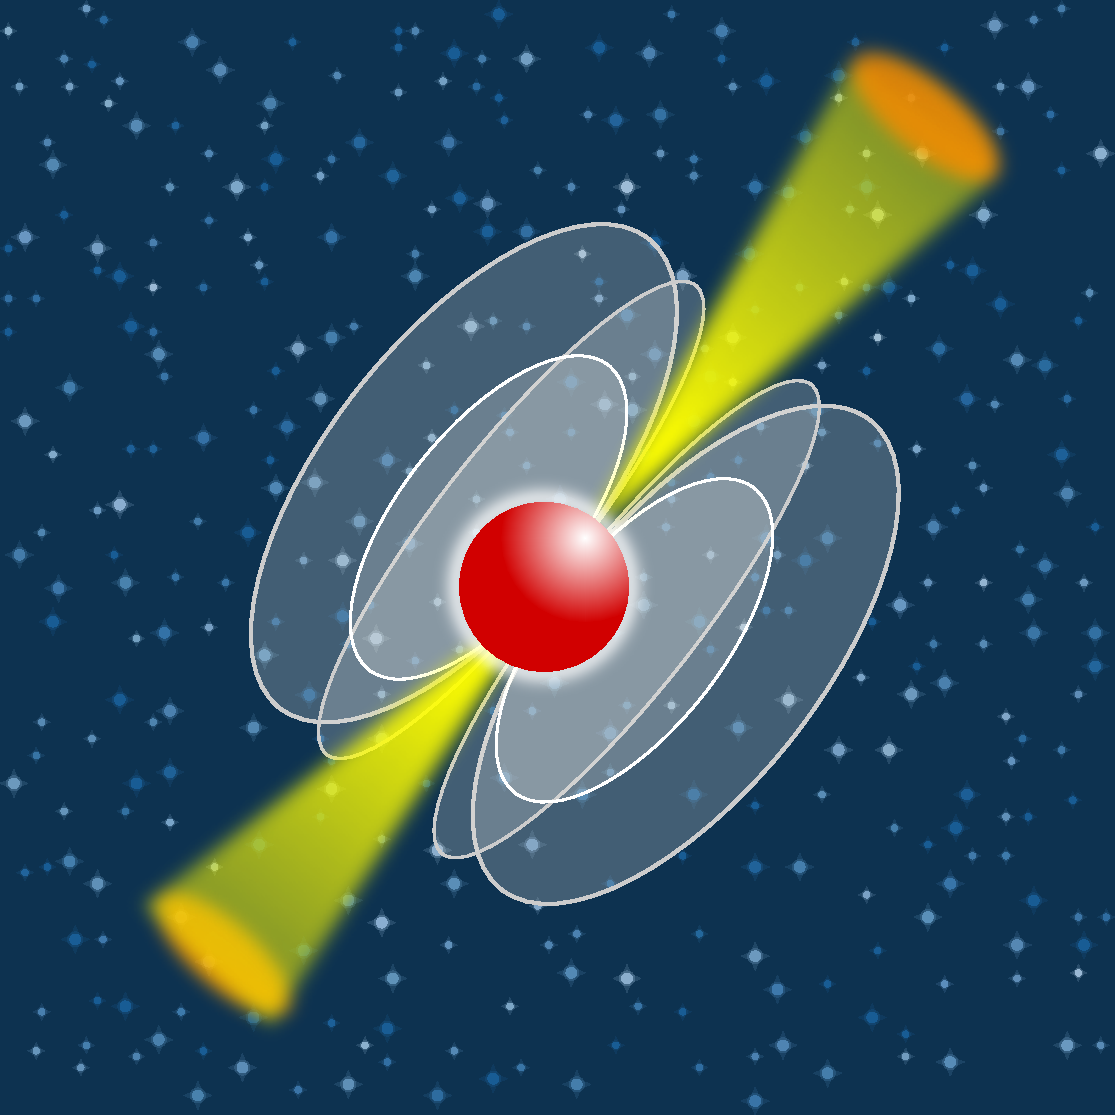
\includegraphics[width=0.88\linewidth,height=0.48\textheight,keepaspectratio]{../figs/pdf/en/fig-05-05.pdf}

% DOCX paragraph 561
\caption{\emph{En un púlsar, la rotación y un campo magnético fuerte aceleran las partículas cerca de los casquetes polares, que emiten radiación colimada (especialmente en la banda de radio). Los haces rotan con la estrella, de forma similar a los de un faro\index{faro}, y pueden «barrer» la Tierra.}}\label{fig:05-05}
\end{figure}

% DOCX paragraph 563
El funcionamiento de un púlsar está representado de forma esquemática en la figura \ref{fig:05-05}, que muestra cómo, en una estrella de neutrones, la acción combinada de una rotación rápida y un fuerte campo magnético\index{dipolo!magnético} produce un fino haz de radiación, mayormente en la banda de radio. La falta de alineación entre el eje de rotación de la estrella y el eje del momento dipolar del campo magnético hace que los haces de radiación roten con la estrella de neutrones, barriendo periódicamente diferentes zonas del cielo.

% DOCX paragraph 564
Así pues, un púlsar es una estrella de neutrones que rota a gran velocidad y emite un haz de luz en la banda de radio, igual que un faro\index{faro} emite un haz de luz en la banda visible. Entonces, cuando a nosotros en la Tierra nos «barre» el haz de luz emitido por la estrella de neutrones, vemos una emisión de radio pulsada, con un periodo de pulsación igual al de la rotación de la estrella (o a la mitad, si podemos ver los dos haces emitidos por los polos del campo magnético).

% DOCX paragraph 565
Un aspecto que hasta ahora solo he mencionado de pasada, pero que en realidad es una de las propiedades fundamentales de las estrellas de neutrones, es la increíble intensidad de su campo magnético\index{estrella de neutrones!campo magnético}: incluso en las más corrientes alcanza valores del orden de 10\textsuperscript{11} o 10\textsuperscript{12} gauss\index{gauss (campo magnético)}. Para compararlo con realidades más próximas a nosotros, el campo magnético de la Tierra, por ejemplo, es de aproximadamente medio gauss, el del Sol de un gauss y el de las barras imantadas (como los imanes que pegamos en el frigorífico) es del orden de unos 100 gauss. En resumen, el campo magnético de una estrella de neutrones normal es un billón de veces más intenso que el que nos encontramos todos los días en nuestro planeta. Pero hay estrellas de neutrones cuyo campo magnético es incluso más intenso y puede alcanzar valores enormes: 10\textsuperscript{14} o 10\textsuperscript{15} gauss, hasta mil veces más intenso que el de un púlsar\index{estrella de neutrones!púlsar (véase)} «normal».

% DOCX paragraph 566
Estas estrellas de neutrones reciben el evocador nombre de \emph{magnetar\index{magnetar}es\index{estrella de neutrones!magnetar (véase)}} y, muy de tarde en tarde, pueden emitir destellos tan potentes en las bandas de rayos X y de radio que, por unos momentos, son capaces de eclipsar a todos los demás objetos celestes juntos. Para que te hagas una idea de la cantidad descomunal de energía\index{energia@energía!emisión} que libera un magnetar cuando emite radiación de manera explosiva, podemos fijarnos en el caso de SGR 1806--20\index{SGR 1806–20}, que registró una de estas explosiones en diciembre de 2004. Los cálculos muestran que la cantidad de energía emitida por esta fuente en tan solo una décima de segundo ¡superó la que ha producido el Sol en los últimos 100\,000 años!

% DOCX paragraph 567
Seguimos sin saber cuál es la causa de estos fenómenos. No obstante, se plantea la hipótesis de que unos cambios repentinos en el equilibrio de la corteza de estas estrellas de neutrones (comparables a terremotos formidables) producen variaciones enormes en el campo magnético de su superficie. Esto, a su vez, libera cantidades inmensas de energía magnética\index{energia@energía!magnética}, que se convierte en radiación\index{rayos X!radiación} de rayos X o gamma. El proceso en sí no es tan inusual, y se observa con regularidad en el Sol, donde da lugar a auténticas explosiones magnéticas, también conocidas como \emph{llamaradas solares\index{Sol!llamarada}}.

% DOCX paragraph 568
Cabría preguntar: «¿Cómo se producen estos campos magnéticos tan intensos?». Pues bien, el origen del enorme campo magnético\index{púlsar!campo magnético} de los púlsares y los magnetar\index{magnetar}es sigue siendo objeto de intensa investigación y debate. Una explicación plausible, aunque no la única, es que se trata de un campo magnético «fósil», es decir, heredado de la estrella original antes de su colapso\index{gravitatorio!colapso}. En este caso, el proceso que interviene es la \emph{conservación del flujo del campo magnético} (o \emph{congelación del flujo\index{congelación del flujo}}) durante el colapso\index{gravitatorio!colapso} gravitatorio que da lugar a la estrella de neutrones. El producto entre la sección de la propia estrella (que es proporcional al cuadrado de su radio) y la intensidad del campo magnético debería ser siempre el mismo. Durante el colapso, la estrella original pasa de un radio de más de un millón de kilómetros a uno de solo diez, de forma que la mera reducción de la sección basta para obtener un factor de amplificación de (100\,000)\textsuperscript{2}=10\,000\,000\,000 veces.

% DOCX paragraph 569
Para comprender lo que sucede, imagina que tomas un imán como los que muchos tenemos en el frigorífico de casa y lo comprimes con una prensa hidráulica hasta reducir su radio a la mitad: de esta manera, su campo magnético aumentará en un factor de cuatro, es decir, 2\textsuperscript{2}. Lo mismo ocurre en una estrella que colapsa. La gran diferencia es que puede partir de un campo magnético muy débil y desarrollar uno enorme debido a la gigantesca reducción del radio que provoca el colapso.

% DOCX paragraph 570
Junto a la hipótesis del origen fósil hay otra: que el increíble campo magnético\index{estrella de neutrones!campo magnético} se genera después del colapso, cuando la estrella de neutrones todavía es un objeto fluido\index{fluido} y extremadamente caliente, sujeto a grandes oscilaciones y en busca de un nuevo equilibrio. En esas condiciones extremas, complejos fenómenos de turbulencia y dinamo magnética dentro de la protoestrella de neutrones pueden amplificar su campo magnético hasta los valores medidos mediante observaciones de radio. Este último panorama, cuyos detalles todavía son difíciles de reproducir mediante simulaciones y estimaciones teóricas, podría explicar los excepcionales campos magnéticos observados en los magnetar\index{magnetar}es.

% DOCX paragraph 571
Para completar la lista de propiedades maravillosas de las estrellas de neutrones ---en el sentido de que no pueden provocarnos otra cosa que puro asombro---, me gustaría enseñarte una más: son unos relojes increíblemente precisos. Para entender cómo es posible, debemos recordar que, gracias a la elevada rotación y a la capacidad de emitir un fino haz de luz de manera exquisitamente periódica, los púlsares son los objetos astronómicos medidos con mayor precisión: la radioastronomía de púlsares es, en efecto, una ciencia de altísima precisión.

% DOCX paragraph 572
Tener a tu disposición una señal que se repite regularmente y con elevada frecuencia te permite recoger, a lo largo de los años, una enorme cantidad de datos con propiedades estadísticas precisas. De esta manera, se pueden reducir los errores sistemáticos que suelen aquejar a las medidas y alcanzar una exactitud excelente. Esta es la razón por la cual el periodo\index{púlsar!periodo} de algunos púlsares se conoce con una precisión de 10\textsuperscript{-15}, o sea, una parte en mil billones (en otras palabras, ¡con una precisión tal que se puede expresar mediante un número del que conocemos exactamente 15 dígitos!). Así ocurre, por ejemplo, con el púlsar de rotación más rápida que conocemos, PSR J0437--4715\index{PSR J0437–4715}: sabemos que su periodo es de 0,005757451936712637 segundos.

% DOCX paragraph 573
Para hacernos una idea de lo exacta que es esta medición, imaginemos la precisión necesaria para identificar, una por una, todas las células presentes en un ser humano, que ascienden a unos treinta billones (aproximadamente 3×10\textsuperscript{13}). Pues bien, el periodo de PSR J0437--4715\index{PSR J0437–4715} se conoce con una precisión ¡cien veces mayor! Si en biología hubiéramos logrado esta precisión, seríamos capaces de «clonar» un ser humano simplemente juntando los treinta billones de células que lo componen…

% DOCX paragraph 574
La increíble precisión con la que podemos medir el periodo de los púlsares también nos dice que podemos utilizarlos como relojes cósmicos extraordinariamente precisos. Para afirmar que un reloj es «bueno», es esencial que tenga un periodo regular, pero es igual de importante que su periodo varíe de una manera constante y predecible. En el caso de los púlsares, cambia de forma casi imperceptible, pero cambia. Así pues, lo que importa, y para nosotros es una suerte, es justamente que varía de forma regular y fácil de predecir.

% DOCX paragraph 575
La razón por la cual el periodo de rotación de un púlsar\index{púlsar!pérdida de energía} tiene que cambiar es bastante fácil de entender. Igual que un faro\index{faro} (que necesita electricidad para funcionar), un púlsar tiene que recurrir a alguna forma de energía para emitir su haz\index{púlsar!haz} de radiación en la banda de radio. Esta «reserva» la constituye su energía cinética. Para ser más exactos, la rotación del púlsar varía y su periodo se hace cada vez más largo porque la estrella pierde parte de su energía cinética de rotación al emitir ondas electromagnéticas\index{ondas!electromagneticas@electromagnéticas} en la banda de radio (lo que se denomina \emph{frenado\index{púlsar!frenado}} del púlsar, o \emph{spin down}). Reconocer este mecanismo es una piedra angular de nuestra comprensión de los púlsares. El astrofísico italiano Franco Pacini\index{Pacini, Franco} fue el primero en sugerir la idea, en 1967 (una vez más, ¡\emph{annus mirabilis}!). Demostró que un púlsar se parece a un dipolo magnético\index{dipolo!magnético} giratorio: en pocas palabras, una barra magnética con un polo norte y un polo sur en rápida rotación. La tasa de cambio de la rotación está relacionada con la cantidad de energía que se pierde.\textsuperscript{\hyperlink{note:05-13}{13}} Es como si la emisión de radiación electromagnética frenara la rotación estelar; incluso se puede medir la fuerza de este freno mediante una combinación del periodo de rotación y su variación a lo largo del tiempo, una medida denominada \emph{índice de frenado\index{púlsar!índice de frenado}}.

% DOCX paragraph 576
Ahora bien, la energía que pierde el púlsar\index{púlsar!frenado} de esta manera representa solo una fracción muy pequeña de la energía cinética disponible. Esta es la razón de que el periodo de otro púlsar, llamado PSR J1603--7202\index{PSR J1603–7202} ---que sabemos que es de 0,0148419520154668 segundos---, aumente tan solo 0,0000005 segundos cada millón de años.\textsuperscript{\hyperlink{note:05-14}{14}} En comparación, un reloj suizo de precisión «pierde» unos siete segundos al día, y un reloj de cuarzo unos diez al año… A estas alturas te habrás percatado de la fascinación que ejercen sobre mí las estrellas de neutrones. Sin embargo, para ser imparcial, debo recordarte que, con la tecnología actual, podemos construir relojes atómicos con precisiones aún mayores que las mencionadas para los púlsares: solo pierden 0,0000001 segundos cada millón de años, cinco veces menos que un púlsar. Por otra parte, también hay que decir que es posible mantener esta precisión solo durante intervalos de tiempo bastante cortos, del orden de unas pocas horas. En cambio, los púlsares pueden mantenerse estables durante cientos de miles de años. ¡Lo cual, en mi opinión, los hace claramente superiores!

% DOCX paragraph 577
Me gustaría concluir anticipando una pregunta que algunos os habréis planteado. Hemos dicho que un púlsar emite un haz colimado de radiación en la banda de radio y que para ello necesita un campo magnético enorme y una rotación suficientemente elevada, pues es la combinación de estos dos elementos lo que produce los gigantescos campos eléctricos capaces de acelerar partículas cargadas. Sin embargo, acabamos de ver que un púlsar gira cada vez más despacio, aunque tarde millones de años en frenarse del todo. Es, por tanto, legítimo preguntarse si, llegado un momento, la rotación de un púlsar puede ser tan lenta que ya no sea capaz de emitir radiación electromagnética. La respuesta es sí: un púlsar puede «apagarse», es decir, disminuir su velocidad hasta el punto de dejar de ser visible como un faro\index{faro}. Cuando esto sucede, se dice que el púlsar ha cruzado la \emph{línea de muerte\index{púlsar!línea de muerte}}. A partir de ese momento, ya no será visible, aunque, obviamente, seguirá girando y tendrá un campo magnético intenso durante miles de millones de años más. Como solo vemos las estrellas de neutrones que aparecen como «púlsares encendidos», ¡creemos que hay muchas más de las que hemos visto hasta ahora!

% DOCX paragraph 580
\section{Un interior misterioso y fascinante}\label{sec:05-interior}

% DOCX paragraph 582
Otra pregunta más que legítima que nos podríamos hacer es esta: «Pero ¿qué aspecto tiene el interior\index{estrella de neutrones!interior} de una estrella de neutrones?».

% DOCX paragraph 583
La respuesta, sin rodeos, se podría resumir así: ¡fundamentalmente, no lo sabemos! En otras palabras, solo tenemos una vaga idea ---o más bien muchas ideas incompatibles entre sí--- de la estructura interna y la composición de una estrella de neutrones. La razón de esta «ignorancia» está a la vista: las condiciones físicas dentro de un objeto así están lejos de las que se pueden poner a prueba y reproducir mediante experimentos de laboratorio. Por tanto, es objetivamente difícil, tanto desde el punto de vista teórico como desde el experimental, extrapolar a partir de lo que conocemos a densidades mucho más bajas (y con un número de partículas enormemente inferior) y llegar a conclusiones válidas para la densidad y la presión que existen dentro de una estrella de neutrones.

% DOCX paragraph 584
Dicho esto, hay aspectos de su composición y su estructura interna en los que todos están de acuerdo. Por ejemplo, está bastante claro que una estrella de neutrones no solo está compuesta por neutrones, sino que también contiene otras partículas (aunque en pequeñas cantidades). Las más importantes son, sin duda, protones y electrones, y estos últimos son responsables, en última instancia, de la producción de los enormes campos magnéticos de los que hemos hablado. Los electrones (y otras partículas cargadas ligeras) son, de hecho, capaces de producir las inmensas corrientes eléctricas necesarias para generarlos. Además, a pesar de la incertidumbre de fondo, está bastante claro que la estructura de una estrella de neutrones debe caracterizarse por zonas específicas cuyos grosores conocemos con cierta precisión. Por otra parte, la presencia de capas también se da en nuestro planeta, cuya física es mucho más sencilla y cuya estructura podemos investigar directamente.

% DOCX paragraph 585
Imaginemos, pues, que «diseccionamos» una estrella de neutrones para comprender su estructura\index{estrella de neutrones!estructura}, empezando por la superficie y desplazándonos hacia el centro. La primera capa que nos encontramos consiste en una especie de atmósfera (y técnicamente se llama así), una piel muy fina, de no más de un centímetro de grosor, compuesta de átomos extremadamente pesados y con una densidad miles de millones de veces superior a la de nuestra atmósfera. Por extremas que sean, las propiedades de esta atmósfera están bastante claras y su física se ha puesto a prueba relativamente bien, hasta el punto de que la consideramos esencialmente «conocida». Resulta paradójico: la única parte de un objeto con un radio de una docena de kilómetros cuyas propiedades creemos conocer en detalle ¡tiene un grosor de no más de un centímetro!

% DOCX paragraph 586
Dirigiéndonos hacia el centro, debajo de la atmósfera hallaremos lo que se denomina la \emph{corteza}. Una capa de uno o dos kilómetros de grosor que contiene iones\index{iones} pesados, es decir, iones con una masa atómica grande, pero también electrones de muy altas energías, llamados por ello \emph{electrones relativista\index{electron@electrón!relativista}s}. Hay que advertir que el término «corteza» puede llamar a engaño, pues se trata de un material elástico y deformable, con cierta similitud con una sustancia plástica extremadamente densa. Sin embargo, parte de la materia de la corteza tendrá todavía las características de una red cristalina, es decir, mostrará una estructura periódica y regular en la cual los iones están a distancias precisas y los electrones se mueven libremente por los espacios vacíos. Este tipo de estructura es la que solemos encontrar en los objetos sólidos y la responsable de sus propiedades mecánicas.

% DOCX paragraph 587
Por debajo de la corteza, en una capa que podría extenderse a lo largo de seis o siete kilómetros, nos encontraremos con el \emph{núcleo externo}; allí, la densidad alcanza billones o decenas de billones (en suma, 10\textsuperscript{13} o 10\textsuperscript{14}) de gramos por centímetro cúbico. Una densidad enorme, pero no la máxima, que encontraremos al avanzar hacia la zona central de la estrella de neutrones, su \emph{núcleo interno}, cuyo grosor también es de seis o siete kilómetros.

% DOCX paragraph 588
Las propiedades de la materia presente en el núcleo\index{estrella de neutrones!núcleo} interno siguen siendo básicamente desconocidas y representan un desafío teórico excepcional al que los físicos nucleares llevan enfrentándose casi cuarenta años. No te sorprenderá saber que abundan las hipótesis al respecto, algunas más conservadoras, otras decididamente menos. Pero quizá la cuestión más importante y fascinante sobre las condiciones\index{iones} físicas en las zonas más profundas de una estrella de neutrones sea la presencia de \emph{partículas exóticas\index{exóticas!partículas}}, como los hiperones o incluso los quarks libres. De estos últimos hablamos en el capítulo 1: son las partículas elementales que constituyen otras partículas, como los neutrones y los protones. Dicho de otra manera, es posible que en el centro de la estrella, como consecuencia de la elevadísima densidad que alcanza el núcleo más interno (cuyo radio no supera un par de kilómetros), los quarks estén tan cerca unos de otros que se «liberen», es decir, que dejen de estar confinados dentro de un neutrón o un protón y formen así una \emph{sopa\index{quark!sopa} de quarks}. Esta hipótesis es particularmente fascinante porque sabemos que una sopa\index{quark!sopa} de este tipo tuvo que estar presente en los primerísimos momentos de la vida del universo (hasta una centésima de segundo), y se produce, aunque solo sea durante intervalos de tiempo muy breves, cuando en los experimentos se hacen chocar iones pesados a energías muy altas. La idea de que esta sopa, en cambio, esté presente de manera estable dentro de las estrellas de neutrones y se pueda revelar de alguna manera (quizá mediante la emisión de ondas gravitatorias) podría abrir campos de investigación que involucren a científicos de todo el mundo, entre los que me incluyo.

% DOCX paragraph 589
Las dudas sobre la composición interna de las estrellas de neutrones, de las que acabamos de hablar, se describen por lo general como una incertidumbre en la llamada \emph{ecuación de estado\index{ecuación de estado}\index{estrella de neutrones!ecuación de estado}}. Para ser precisos, cuando los físicos hablan de la ecuación de estado de una estrella de neutrones, se refieren a la capacidad de comprender cómo varía la presión (y, por tanto, la composición interna) de un objeto así al pasar de la superficie al centro. La incertidumbre al respecto también se traduce en una incertidumbre ---particularmente grave desde el punto de vista de la observación--- sobre el tamaño que puede tener una estrella de neutrones. Hasta hace unos pocos años, las estimaciones de los radios de estos cuerpos celestes cubrían un intervalo bastante amplio: desde los siete kilómetros, calculados con ecuaciones de estado que predicen estrellas muy compactas y que se llaman \emph{ecuaciones de estado blanda\index{ecuación de estado!blanda}s}, hasta los 18 kilómetros de aquellas que predicen estrellas comparativamente más grandes y se conocen como \emph{ecuaciones de estado rígida\index{ecuación de estado!rígida}s}.

% DOCX paragraph 590
Por fortuna, hoy tenemos toda una serie de observaciones ---tanto en el canal electromagnético como en el de ondas gravitatorias--- que nos proporcionan indicaciones más precisas sobre el radio de una estrella de neutrones de 1,4 masas solares (que se suele considerar la masa de referencia): de hecho, se espera que esté entre diez y 14 kilómetros. En cualquier caso, la determinación del radio de las estrellas de neutrones es un campo de investigación muy activo, en el que también participo. Además, cada vez que un nuevo instrumento proporciona nuevas medidas o cuando se detecta la fusión de un sistema binario de estrellas de neutrones, se proponen nuevas estimaciones. Por tanto, ¡no se puede descartar que las estimaciones anteriores pronto queden obsoletas!

% DOCX paragraph 593
\section{Masa máxima}\label{sec:05-mass}

% DOCX paragraph 595
La idea mencionada anteriormente de un radio típico para una masa de referencia me permite introducir un aspecto que hasta ahora había dejado de lado al presentar las propiedades de las estrellas de neutrones, a pesar de que es el tema principal de este libro: la gravedad producida por un cuerpo celeste como este.

% DOCX paragraph 596
También desde este punto de vista, una estrella de neutrones\index{compacidad!estrella de neutrones} es un objeto con características extremas. La gravedad que genera es, de hecho, al menos mil millones de veces más intensa que la que tenemos en la Tierra. Si, por absurdo que resulte, aterrizáramos en su superficie, la gravedad reduciría nuestra nave espacial ---y a nosotros dentro de ella--- a un objeto casi bidimensional: quedaríamos extendidos sobre una superficie reticular cuya extensión vertical no superaría un puñado de átomos. Además, dado que la compacidad\index{estrella de neutrones!compacidad} típica de una estrella de neutrones varía entre \emph{M/R} = 0,17 y \emph{M/R} = 0,25, está claro que se trata de curvaturas, cuando menos, muy significativas, que dan lugar a efectos relativistas muy intensos, como la dilatación del tiempo o la curvatura de las trayectorias de la luz.\index{dilatación del tiempo}

% DOCX paragraph 597
Hay, sin embargo, un aspecto particular de la relación entre gravedad y estrellas de neutrones que es una consecuencia directa de la teoría de la relatividad general: la existencia de una \emph{masa máxima\index{estrella de neutrones!masa máxima}}. Para comprender de qué se trata, es necesario hacer referencia a las soluciones de las ecuaciones de Einstein que nos permiten construir modelos de estrellas de neutrones en equilibrio\index{equilibrio}. En esencia, tras elegir una ecuación de estado\index{ecuación de estado} que vincule la presión dentro de la estrella con la densidad local de la materia, se pueden resolver las ecuaciones de Einstein y encontrar un modelo de equilibrio que represente una estrella de neutrones. Llegados ahí, al variar la masa de la estrella, se puede obtener una «secuencia» de modelos, es decir, el conjunto de estrellas de neutrones que corresponden a una determinada ecuación de estado. Como no conocemos la ecuación de estado correcta, podemos construir numerosas secuencias de este tipo ---yo he construido casi dos millones---, todas ellas físicamente plausibles.

% DOCX paragraph 598
Todas estas secuencias comparten una propiedad: el radio estelar disminuye al aumentar la masa. Si lo piensas, se trata de un comportamiento bastante anómalo en astrofísica: estamos acostumbrados a encontrar objetos en los cuales una masa mayor corresponde también a un radio mayor; basta pensar en lo que ocurre con las estrellas normales o los planetas. Sin embargo, en las condiciones extremas de densidad y presión que caracterizan las estrellas de neutrones, ocurre lo contrario: al aumentar la masa, el radio tiende a disminuir.

% DOCX paragraph 599
La figura \ref{fig:05-06} muestra una gráfica esquemática de la relación entre masa y radio en una estrella de neutrones genérica. La masa (expresada en masas solares) se sitúa en el eje vertical, y el radio (expresado en kilómetros), en el horizontal. La línea negra continua representa el conjunto de soluciones de las ecuaciones de Einstein para una determinada ecuación de estado, de manera que cada uno de sus puntos es una configuración en equilibrio estable\index{equilibrio!estable}. Como puede verse, el radio tiende a disminuir al aumentar la masa, pero esta última no puede crecer indefinidamente. La curva negra tiene un máximo, indicado con un punto, más allá del cual la línea es discontinua: es la llamada \emph{rama inestable\index{rama inestable}\index{equilibrio!inestable}} de las configuraciones de equilibrio. En otras palabras, aunque también es posible hallar soluciones de las ecuaciones de Einstein en la parte discontinua de la línea, están sujetas a una «inestabilidad gravitatoria\index{inestabilidad!gravitatoria}» y, por tanto, son inestables. Las estrellas de neutrones correspondientes colapsarían bajo la atracción gravitatoria.

% DOCX paragraph 600
Por tanto, cada ecuación de estado\index{ecuación de estado} tiene una masa máxima, con una rama estable y otra inestable de soluciones de equilibrio\index{equilibrio}; la franja gris que rodea la curva negra representa así la incertidumbre introducida al determinar el radio de una estrella de neutrones por desconocer su estructura interna. Si la ecuación de estado fuera única y conocida, esa franja se reduciría hasta coincidir con la línea negra. Entonces sería posible conocer exactamente el radio, la estructura y la composición interna de la estrella una vez fijada su masa, quizá mediante observaciones (como ejemplifica la línea horizontal de puntos). De hecho, las observaciones nos proporcionan medidas muy precisas de la masa, pero no logran revelarnos directamente el radio.\index{rama inestable}

% DOCX paragraph 603
\begin{figure}[htbp]
\centering
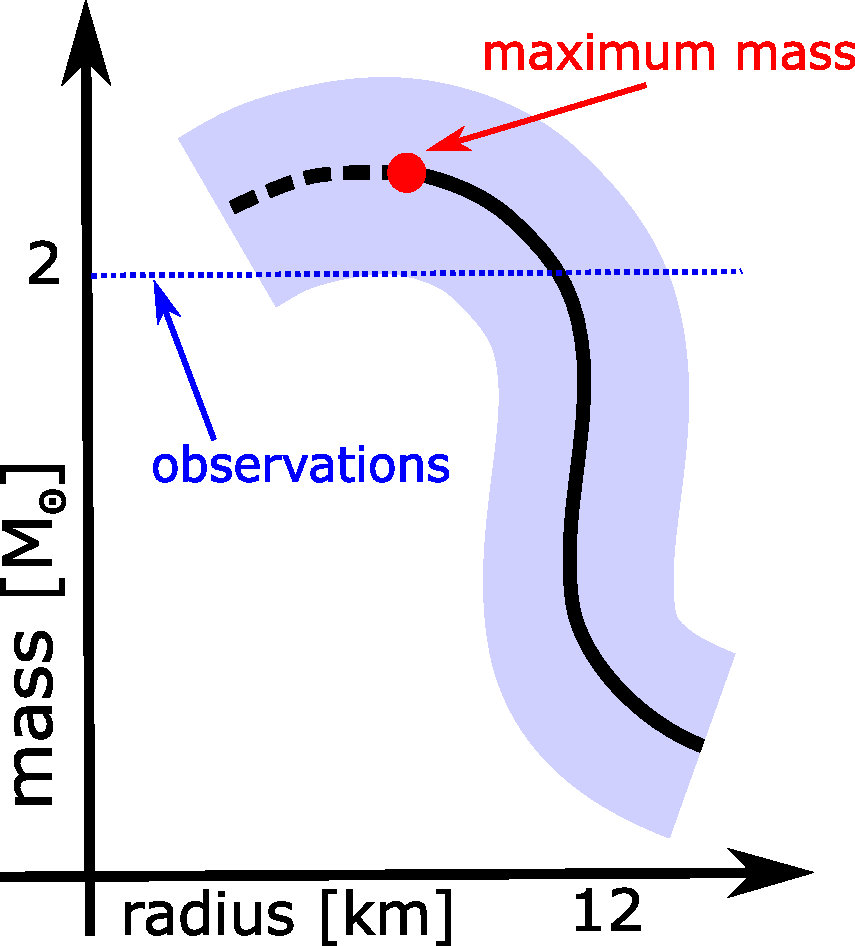
\includegraphics[width=0.88\linewidth,height=0.48\textheight,keepaspectratio]{../figs/pdf/en/fig-05-06.pdf}

% DOCX paragraph 605
\caption{\emph{Relación entre masa y radio en una estrella de neutrones. El radio disminuye al aumentar la masa, y alcanza un mínimo en la masa máxima. Las estrellas con masas mayores colaps\index{gravitatorio!colapso}arían, de modo que no son posibles.}}\label{fig:05-06}
\end{figure}

% DOCX paragraph 607
Llegados a este punto, me gustaría invitarte a realizar otro experimento mental. Consideremos una estrella de neutrones\index{estrella de neutrones!masa máxima} con una masa muy próxima a su máximo: en la gráfica estará casi en la cima de la curva continua, ligeramente a la derecha y por debajo del punto rojo. Esta estrella sería perfectamente estable: si la perturbáramos con un buen martillazo en su superficie, respondería oscilando de manera estable, aunque amortiguada. Sin embargo, si aumentáramos su masa, siquiera en una cantidad infinitesimal, por ejemplo añadiendo un solo neutrón, la llevaríamos más allá del punto crítico, donde sería inestable. Su masa superaría el máximo permitido por la ecuación de estado y, por tanto, se vería obligada a hacer algo muy distinto de oscilar: colaps\index{gravitatorio!colapso}aría sobre sí misma.

% DOCX paragraph 608
La teoría de la gravedad de Newton no prevé un límite máximo de masa: según ella, siempre es posible añadir un poco de materia a una estrella. Tampoco contempla la física newtoniana el colapso gravitatorio de una estrella de neutrones con masa «excesiva»: es el resultado de la existencia de soluciones adicionales a las de las estrellas de neutrones, y hablaremos de ello en el próximo capítulo. Por ahora no conocemos el valor de esa masa máxima. Pero hay un púlsar, PSR J0348+0432\index{PSR J0348+0432}, cuya masa se ha medido con gran precisión y resulta ser de 2,01 ± 0,04 masas solares. Del hecho de que exista en la naturaleza una estrella de neutrones con una masa tan elevada se deduce que la masa máxima debe ser necesariamente mayor (como se muestra en la figura \ref{fig:05-06}).

% DOCX paragraph 609
Además, la reciente observación de la fusión de un sistema binario\index{estrella de neutrones!binaria (véase)} de estrellas de neutrones ---GW170817\index{GW170817}--- ha proporcionado datos para nuevas hipótesis sobre este límite. Actualmente, muchos científicos ---yo entre ellos, como argumenté en un artículo aparecido hace un par de años--- piensan que la masa máxima probablemente está por debajo de 2,33 masas solares. En otras palabras, la escurridiza masa máxima de una estrella de neutrones se sitúa ahora razonablemente entre 2,0 y 2,3 masas solares. Por desgracia, aunque se trata de un intervalo bastante estrecho, sigue sin permitirnos tener una idea precisa de la estructura y la composición interna de una estrella de neutrones. Sin embargo, las observaciones de los próximos años nos proporcionarán muchas otras indicaciones que nos ayudarán a acotar mejor su valor.

% DOCX paragraph 610
Para concluir esta digresión sobre la masa máxima, y a modo de aperitivo de lo que trataremos a continuación, déjame anticiparte que, para comprender lo que le ocurre a una estrella de neutrones con una masa superior a la máxima y, por tanto, condenada al colapso\index{gravitatorio!colapso} por ser gravitatoria\index{inestabilidad!gravitatoria}mente \emph{inestable}, necesitamos entender el estado final al que se llega mediante ese colapso. Es decir, el de un agujero negro, al que dedicamos el capítulo 6.

% DOCX paragraph 613
\section{¿Quién teme a una estrella de neutrones?}\label{sec:05-danger}

% DOCX paragraph 615
A lo largo de los últimos cincuenta años, las estrellas de neutrones, y los púlsares en particular, han sido objeto de campañas de observación intensas e ininterrumpidas. Por esta razón, ahora conocemos más de 2800 púlsares, y toda la información al respecto está disponible gratuitamente en internet a través del catálogo compilado y actualizado por la Australian Telescope National Facility (o, simplemente, ATNF). Aun así, las estrellas de neutrones observadas hasta ahora no son más que la punta del iceberg: solo en la Vía Láctea\index{Vía Láctea}, su población estimada varía entre doscientas mil y un millón. La mayoría de estos púlsares están aislados, es decir, no están asociados con otras estrellas, pero también hay una fracción considerable en sistemas binarios, en los que una estrella normal acompaña a la estrella de neutrones.

% DOCX paragraph 616
Justamente eso es lo que ocurre con Sco X-1\index{Scorpius X-1 (Sco X-1)} ---el punto de partida de este capítulo---, donde la estrella de neutrones arranca materia de la secundaria y la hace caer sobre sí en forma de disco de acreción\index{disco de acreción}. Cuando la materia robada a la compañera cae sobre la estrella de neutrones, el enorme salto gravitatorio que experimenta (¿recuerdas las centrales hidroeléctricas?) hace que se caliente hasta alcanzar temperaturas de un millón de kelvin, y produce así la emisión de rayos X\index{rayos X!radiación} que nos permitió descubrirla.

% DOCX paragraph 617
¡Pero los sistemas binarios de este tipo pueden alcanzar temperaturas aún mayores! Si lo piensas, la materia depositada en la superficie de la estrella de neutrones también tiene que ir a parar a algún sitio. Por lo que sabemos hoy, se acumula en una capa de solo unos pocos centímetros de grosor (no olvidemos que la gravedad en la superficie de una estrella de neutrones es enorme). Como las partes exteriores de una estrella normal están compuestas de elementos ligeros como el hidrógeno y el helio, la transferencia de materia de la estrella normal a la de neutrones solo deposita materia de baja masa atómica (hidrógeno o helio), que es, por tanto, muy «combustible» mediante fusión termonuclear\index{fusion termonuclear@fusión termonuclear}. Así pues, a medida que la materia arrancada se acumula y se calienta sobre la superficie de la estrella de neutrones, se pueden alcanzar las condiciones adecuadas de densidad y temperatura para que en esa fina piel se desencadene una reacción de fusión termonuclear, que literalmente destruye la capa acumulada y la hace elevarse de la superficie en una deslumbrante esfera de luz.

% DOCX paragraph 618
Esta enorme explosión nuclear, que involucra una porción considerable de toda la superficie de la estrella de neutrones, libera una cantidad de energía equivalente a casi un trillón de bombas atómicas. Además, esta gigantesca liberación de energía se produce en una escala temporal de entre uno y diez segundos. Da lugar al proceso que los astrónomos llaman \emph{estallido de rayos X\index{estrella de neutrones!estallido de rayos X}\index{rayos X!radiación}}, que caracteriza, de manera más o menos regular, la emisión de las fuentes en sistemas binario\index{púlsar!binario}s de rayos X\index{rayos X!radiación} de baja masa (LMXB). Las estrellas de neutrones no solo se han observado en estos sistemas, sino que también están presentes en otras configuraciones y, en particular, en sistemas binarios compuestos por dos estrellas de neutrones. Una subclase especial la representan aquellos sistemas en los que ambas estrellas de neutrones son también púlsares, y que por ello reciben el nombre de \emph{púlsares binarios\index{estrella de neutrones!púlsares binarios}}. Volveremos a ellos en el capítulo 8, cuando descubramos que representan fuentes extremadamente intensas de ondas gravitatorias y unos laboratorios riquísimos para estudiar las propiedades de la gravedad en campos muy intensos.

% DOCX paragraph 619
Pero quiero concluir este capítulo con una pregunta lógica, que quizá ya te hayas hecho dadas las características extremas, en todos los sentidos, de las estrellas de neutrones: «¿Deberíamos tener miedo de estos objetos celestes?».

% DOCX paragraph 620
Igual que ocurre con cualquier fenómeno natural de gran belleza y potencia, como un volcán en erupción, también es recomendable observar las estrellas de neutrones desde una «distancia de seguridad»: sus propiedades pueden resultar decididamente peligrosas para seres tan frágiles como nosotros. No obstante, la estrella de neutrones más cercana, RXJ1856.5--3754\index{RX J1856.5–3754}, está a una distancia de 500 años luz (recordemos que la estrella normal más próxima, aparte del Sol, está a solo 4,24 años luz de nosotros: Próxima Centauri\index{Proxima Centauri@Próxima Centauri}). Además, las estrellas de neutrones no son estáticas; de hecho, suelen desplazarse a velocidades muy altas (entre 200 y 400 km/s), que adquieren durante la explosión de supernova que las hace nacer. La emisión de neutrino\index{neutrino!emisión anisótropa}s en los primeros milisegundos de vida de la protoestrella es muy anisótropa\index{anisótropa (emisión de neutrinos)} (es decir, tiene distintas intensidades en distintas direcciones), y esto hace que la protoestrella experimente un «retroceso» en una dirección dada, en la que seguirá vagando durante el resto de su existencia.

% DOCX paragraph 621
Ahora bien, si una estrella de neutrones como RXJ1856.5--3754\index{RX J1856.5–3754} atravesara el sistema solar, incluso sin chocar con ninguno de sus planetas (recordemos que es un objeto diminuto que, comparado con la escala de los demás cuerpos celestes del sistema solar, sería esencialmente un punto apenas mayor que un asteroide), crearía una considerable perturbación gravitatoria debido a su imponente masa, desde luego mayor que la del Sol. Desbarataría algunas de las órbita\index{orbita@órbita}s de nuestro sistema solar y, si pasara cerca de uno de los planetas, por ejemplo Júpiter (el mayor), sencillamente lo destruiría por las enormes fuerzas de marea\index{fuerzas de marea} que desarrollaría.

% DOCX paragraph 622
Además, si un magnetar explotara cerca de nosotros y nos sometiera a una radiación\index{rayos X!radiación} de altísima energía, bastaría para borrar en pocos segundos toda la vida de la Tierra. Esto ocurriría incluso en aquellas zonas del planeta que quedaran a la sombra de las emisiones de rayos X: las inundaría la radiación reflejada por otros planetas o por la Luna\index{Luna}. En otras palabras, creo que todos podemos estar de acuerdo en que sería aconsejable evitar un encuentro demasiado íntimo con una estrella de neutrones, sobre todo si está emitiendo mucha radiación.

% DOCX paragraph 623
Dicho lo cual, tenemos poco de lo que preocuparnos: los magnetar\index{magnetar}es de nuestra galaxia son conocidos y están todos muy lejos de nosotros. Incluso si el púlsar RXJ1856.5--3754\index{RX J1856.5–3754} se dirigiera directamente hacia la Tierra a la máxima velocidad permitida para una estrella de neutrones, no llegaría antes de seis millones de años. Así pues, al menos por ahora, nada tenemos que temer de las estrellas de neutrones y, en cambio, podemos disfrutar de las maravillas que nos revelan.
